\documentclass[12pt,a4paper]{article}
\usepackage[utf8x]{inputenc}
\usepackage[english,hebrew]{babel}
\usepackage{graphicx}
\usepackage{verbatim}
\usepackage{url}
\usepackage{bm}

\graphicspath{{images/}}

\usepackage{tikz}
\usetikzlibrary{external,intersections,patterns}
\tikzexternalize[prefix=tikz/]

% Use stealth arrows
\tikzset {
  >=stealth
}

\textwidth=15.5cm
\textheight=23cm
\topmargin=0pt
\headheight=0pt
\oddsidemargin=2em
\headsep=0pt
\parindent=0pt
\renewcommand{\baselinestretch}{1.1}
\setlength{\parskip}{0.3\baselineskip plus 1pt minus 1pt}

\newcommand{\bover}[1]{\bm{\overline{#1}}}

\begin{document}
\thispagestyle{empty}

\selectlanguage{hebrew}

\begin{center}
\textbf{\Huge מסתבר שלא כל כך קשה\\\mbox{}\\לפתור בעיות בהסתברות}

\bigskip
\bigskip
\bigskip

\textbf{\Large מוטי בן-ארי}

\bigskip

\textbf{\Large מכון ויצמן למדע}

\bigskip

\url{http://www.weizmann.ac.il/sci-tea/benari/}

\bigskip

\end{center}

\selectlanguage{english}

\vfill

\begin{center}
\sffamily\copyright{}\  2018 by Moti Ben-Ari.
\end{center}

\begin{footnotesize}
\sffamily
This work is licensed under the Creative Commons Attribution-ShareAlike 3.0 Unported License. To view a copy of this license, visit \url{http://creativecommons.org/licenses/by-sa/3.0/} or send a letter to Creative Commons, 444 Castro Street, Suite 900, Mountain View, California, 94041, USA.
\end{footnotesize}

\begin{center}

\includegraphics[width=.2\textwidth]{../by-sa.png}
\end{center}

\newpage
\selectlanguage{hebrew}


במסמך נפתור את השאלות על הסתברות בבחינות הבגרות, שאלון
$806$.
מצאתי שהבעיות עצמן קלות יחסית, בתנאי שמבינים את ניסוחי השאלות ואיך לתרגם אותם לחישובים המתאימים. בסוף המסמך סיכמתי את הניסוחים שמופיעים בשאלות.


%%%%%%%%%%%%%%%%%%%%%%%%%%%%%%%%%%%%%%%%%%%%%%%%%%%%%%%%%%%%%%%%%%%


\textbf{\R{
חורף תשע"ח
}}

\begin{center}
\selectlanguage{english}
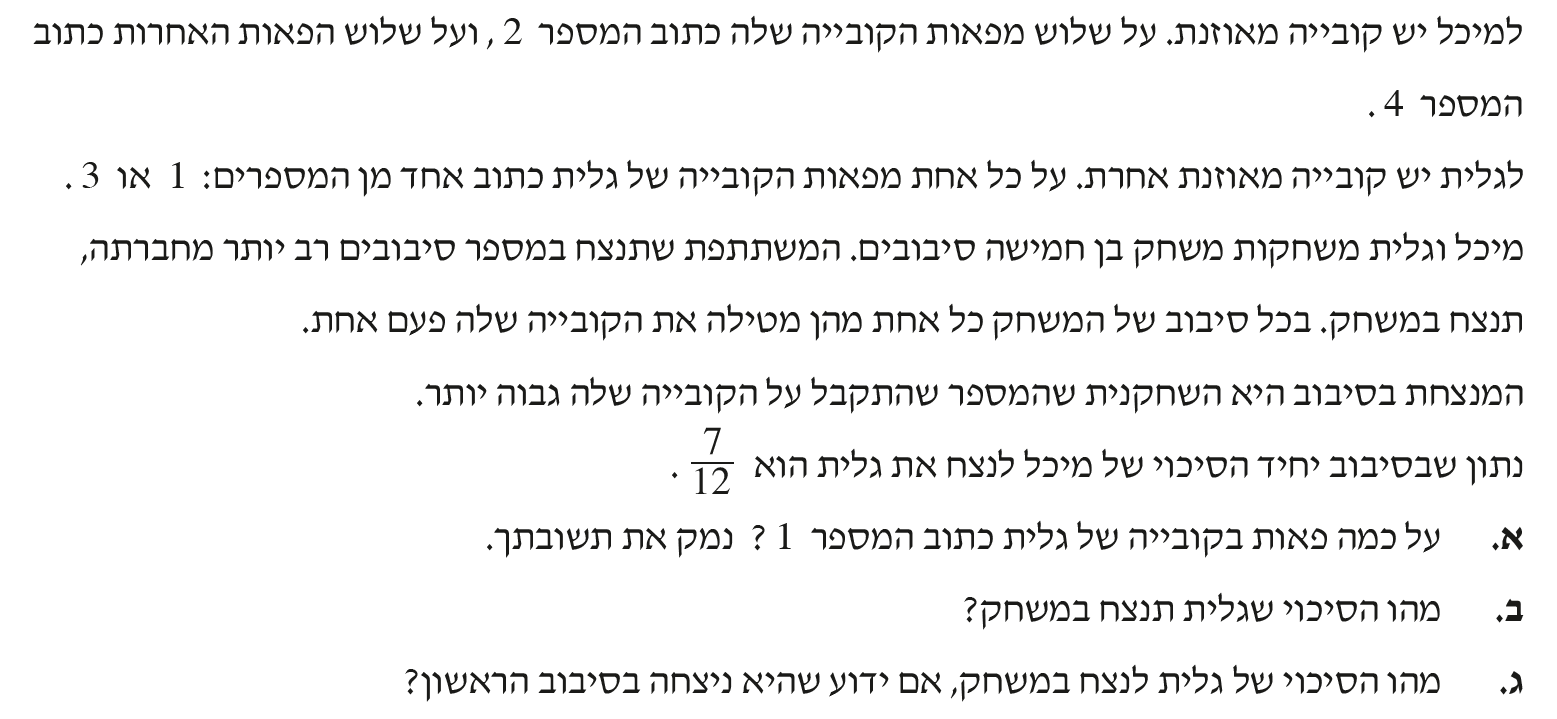
\includegraphics[width=\textwidth]{winter-2018-3}
\end{center}

סעיף א. מיכל תנצח אם )א( היא מטילה 
$4$,
לא משנה מה גלית מטילה אירוע שההסתברות שלה היא 
$1$,
או )ב( מיכל מטילה 
$2$
וגלית מטילה
$1$
אירוע שההסתברות שלה מיא
$\frac{n}{6}$,
כאשר נסמן ב-%
$n$
את המספר הפאות של הקוביה של גלית שכתוב עליהן
$1$.
המשוואה לניצחון של מיכל היא:
\[
\frac{3}{6}\cdot 1 + \frac{3}{6}\cdot \frac{n}{6}=\frac{7}{12}\,,
\]
והפתרון הוא
$n=1$.

סעיף ב. גלית תנצח במשחק אם היא תנצח ב-%
$3,4,5$
סיבובים. לפי נוסחת ברנולי:
\[
{5\choose 3}\left(\frac{5}{12}\right)^3\left(\frac{7}{12}\right)^2+{5\choose 4}\left(\frac{5}{12}\right)^4\left(\frac{7}{12}\right)^1+{5\choose 5}\left(\frac{5}{12}\right)^5\left(\frac{7}{12}\right)^0=0.3466\,.
\]

סעיף ג. המילים 
\textbf{אם ידוע}
מכוונות להסתברות מותנית, כאשר החילוק מצטמצם כי האירועים של הטלת הקובייה בלתי תלויים:
\vspace{-2ex}
\[
\renewcommand{\arraystretch}{2.4}
\begin{array}{c}
P(\textrm{\R{גלית תנצח}}/\textrm{\R{גלית ניצחה בסיבוב הראשון}}) =\\
\displaystyle\frac{P(\textrm{\R{גלית תנצח}}\cap\textrm{\R{גלית ניצחה בסיבוב הראשון}})}{P(\textrm{\R{גלית ניצחה בסיבוב הראשון}})}\\
\displaystyle\frac{P(\textrm{\R{גלית תנצח}})\cdot P(\textrm{\R{גלית ניצחה בסיבוב הראשון}})}{P(\textrm{\R{גלית ניצחה בסיבוב הראשון}})}=\\
P(\textrm{\R{גלית תנצח}})\,.
\end{array}
\]
לאחר הניצחון בסיבוב הראשון, גלית תנצח במשחק אם היא תנצח בשניים מהסיבובים הנותרים:
\[
{4 \choose 4}\left(\frac{5}{12}\right)^4 \left(\frac{7}{12}\right)^0+
{4 \choose 3}\left(\frac{5}{12}\right)^3 \left(\frac{7}{12}\right)^1+
{4 \choose 2}\left(\frac{5}{12}\right)^2 \left(\frac{7}{12}\right)^2
=0.5534\,.
\]


%%%%%%%%%%%%%%%%%%%%%%%%%%%%%%%%%%%%%%%%%%%%%%%%%%%%%%%%%%%%%%%%%%%

\textbf{\R{
קיץ תשע"ח, מועד א
}}

\begin{center}
\selectlanguage{english}
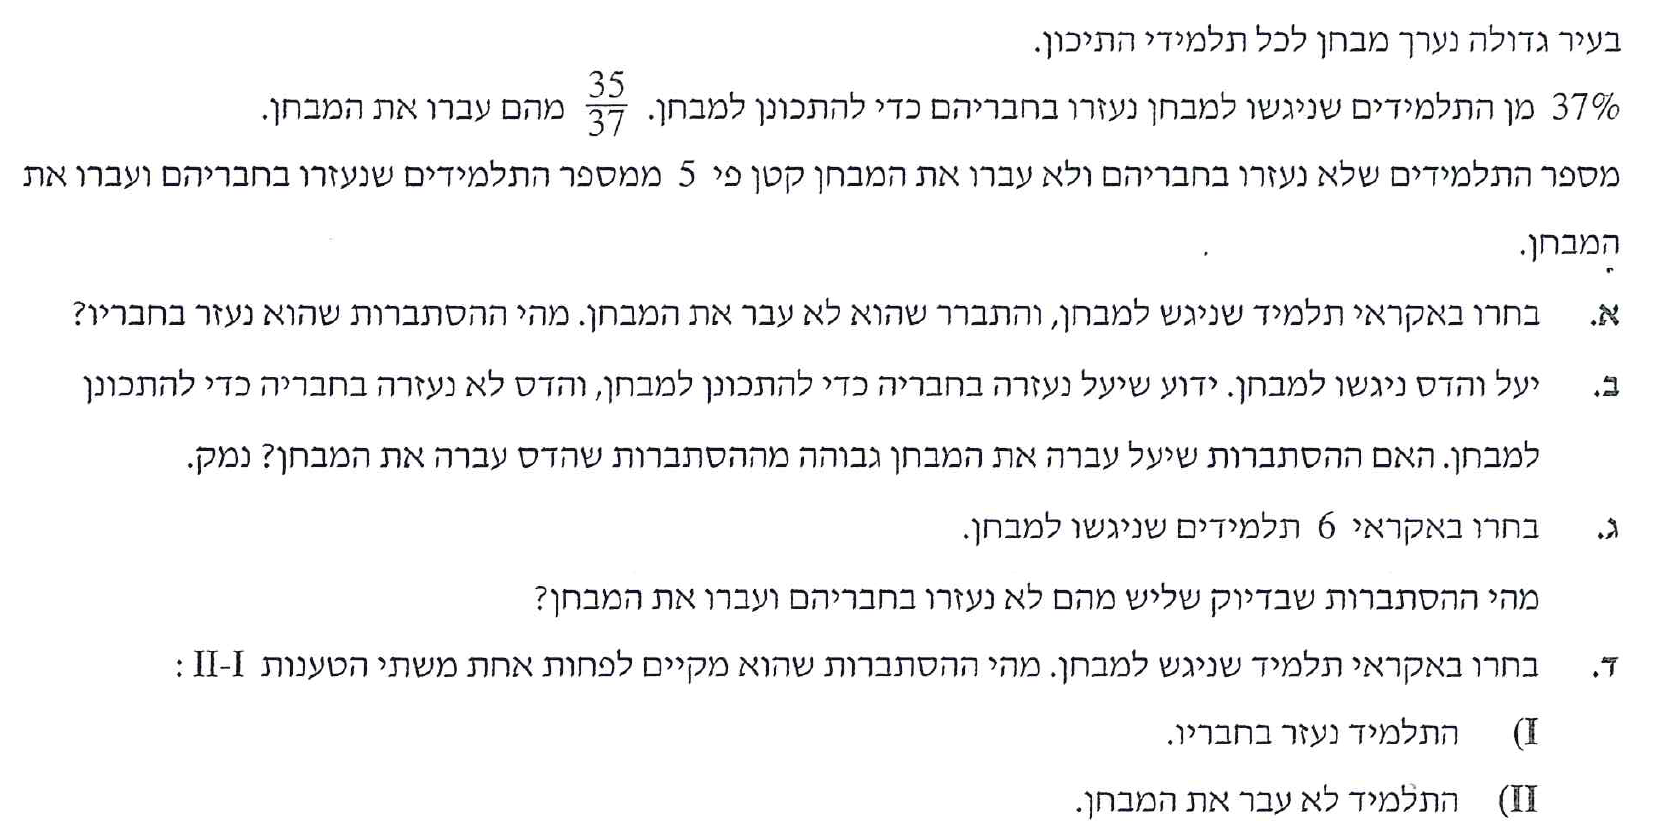
\includegraphics[width=\textwidth]{summer-2018a-3}
\end{center}
נסמן ב-%
$N$
את התלמידים שנעזרו בחבריהם, וב-%
$A$
את התלמידים שעברו את המבחן. נתון ש-%
$P(N)=0.37$.
\textbf{מהם}
עברו את הבחינה 
$\displaystyle\frac{35}{37}$.
זו ההסתברות המותנית
$P(A/N)$.
נחשב:
\[
P(A/N) = \frac{P(N\cap A)}{P(N)} = \frac{P(N\cap A)}{0.37}=\frac{35}{37},\quad\quad\quad P(N\cap A)=0.35\,.
\]
עד כאן טבלת ההסתברויות היא:
\begin{center}
\selectlanguage{english}
\begin{tikzpicture}[scale=1.25]
\draw (0,0) grid (3,3);
\node at (2.5,3.3) {$\bm{A}$};
\node at (1.5,3.3) {$\bover{A}$};
\node at (3.3,2.5) {$\bm{N}$};
\node at (3.3,1.5) {$\bover{N}$};
\node at (2.5,2.5) {$0.35$};
\node at (0.5,2.5) {$0.37$};
\node at (1.5,2.5) {$0.02$};
\node at (0.5,1.5) {$0.63$};
\node at (0.5,0.5) {$1.0$};
\end{tikzpicture}
\end{center}
בהמשך נתון ש-%
\[
P(\overline{N}\cap\overline{A})=\frac{P(N\cap A)}{5}=\frac{0.35}{5}=0.07\,,
\]
וניתן להשלים את הטבלה:
\begin{center}
\selectlanguage{english}
\begin{tikzpicture}[scale=1.25]
\draw (0,0) grid (3,3);
\node at (2.5,3.3) {$\bm{A}$};
\node at (1.5,3.3) {$\bover{A}$};
\node at (3.3,2.5) {$\bm{N}$};
\node at (3.3,1.5) {$\bover{N}$};
\node at (2.5,2.5) {$0.35$};
\node at (0.5,2.5) {$0.37$};
\node at (1.5,2.5) {$0.02$};
\node at (0.5,1.5) {$0.63$};
\node at (0.5,0.5) {$1.0$};
\node at (1.5,0.5) {$0.09$};
\node at (2.5,0.5) {$0.91$};
\node at (1.5,1.5) {$0.07$};
\node at (2.5,1.5) {$0.56$};
\end{tikzpicture}
\end{center}
סעיף א.
\[
P(N/\overline{A})=\frac{P(N\cap \overline{A})}{P(\overline{A})}=\frac{0.02}{0.09}=\frac{2}{9}\,.
\]
סעיף ב. עבור יעל:
\[
P(A/N)=\frac{P(A \cap N)}{P(N)}=\frac{0.35}{0.37}=0.9459\,,
\]
ועבור הדס:
\[
P(A/\overline{N})=\frac{P(A\cap \overline{N})}{P(\overline{N})}=\frac{0.56}{0.63}=0.8889\,.
\]
ליעל סיכוי טוב יותר לעבור את המבחן.

סעיף ג. שליש של שש הוא שניים. )שימו לב שלא לקרוא "שלושה" במקום "שליש"!( החישוב הוא לפי נוסחת ברנולי כאשר הערך של
$P(\overline{N}\cap A)$
נמצא בטבלה:
\[
{6 \choose 2}(0.56)^2 (1-0.56)^4=0.1763\,.
\]
סעיף ד. הניסוח "%
\textbf{לפחות אחת}
משתי הטענות
$I, II$"
אומר שהאירוע קורה אם קורה אחד מהאירועים
$I, II$
\textbf{או שניהם}.
באיור להלן שני עגולים המייצגים את שני האירועים
$I, II$.
האירוע "לפחות אחד משניהם" מיוצג על ידי כל השטח המקווקו.
\begin{center}
\selectlanguage{english}
\begin{tikzpicture}
\begin{scope}
\clip[draw] (0,0) circle[radius=2];
\foreach \y in {-1.5,-1,-.5,0,.5,1,1.5}
  \draw (-2,\y) -- (2,\y);
\end{scope}
\begin{scope}
\clip[draw] (2.5,0) circle[radius=2];
\foreach \x in {1,1.5,2,2.5,3,3.5,4}
  \draw (\x,-2) -- (\x,2);
\end{scope}
\node at (-2,2.5) {$I$};
\node at (4.5,2.5) {$II$};
\node at (1.25,2.5) {$I\cap II$};
\node at (-3.5,.2) {$I/ II$};
\node at (6,.2) {$II/ I$};
\draw[->] (1.25,2.2) -- ++(0,-1);
\draw[->] (-3,.2) -- ++(1.7,0);
\draw[->] (5.5,.2) -- ++(-1.7,0);
\draw[->] (-2,2.2) -- +(.6,-.6);
\draw[->] (4.5,2.2) -- +(-.6,-.6);
\end{tikzpicture}
\end{center}
יש שתי דרכים לחשב את ההסתברות. בדרך הראשונה אנו לוקחים את סכום ההסתברויות של שני האירועים ואז מחסירים את ההסתברות של האירוע המשותף כי ספרנו אותו פעמיים, פעם כחלק מהאירוע I ופעם כחלק מהאירוע II:
\[
P(I \cup II) = P(I) + P(II) - P(I \cap II)\,.
\]
בדרך השניה אנו סופרים כל חלק מהאירוע השותף בנפרד:
\[
P(I \cup II) = P(I/ II) + P(II/ I) + P(I \cap II)\,.
\]
את ההסתברויות לחישוב ניקח מהטבלה. הדרך הראשונה מופיעה מימין והדרך השניה משמאל:
\begin{center}
\selectlanguage{english}
\begin{tikzpicture}[scale=1.25]
\begin{scope}
\draw (0,0) grid (3,3);
\node at (2.5,3.3) {$\bm{A}$};
\node at (1.5,3.3) {$\bover{A}$};
\node at (3.3,2.5) {$\bm{N}$};
\node at (3.3,1.5) {$\bover{N}$};
\node at (2.5,2.5) {$0.35$};
\node at (0.5,2.5) {$0.37$};
\node at (1.5,2.5) {$0.02$};
\node at (0.5,1.5) {$0.63$};
\node at (0.5,0.5) {$1.0$};
\node at (1.5,0.5) {$0.09$};
\node at (2.5,0.5) {$0.91$};
\node at (1.5,1.5) {$0.07$};
\node at (2.5,1.5) {$0.56$};
\draw[ultra thick] (2,2) rectangle +(1,1);
\draw[ultra thick] (1,1) rectangle +(1,1);
\draw[ultra thick] (1,2) rectangle +(1,1);
\end{scope}
\begin{scope}[xshift=6cm]
\draw (0,0) grid (3,3);
\node at (2.5,3.3) {$\bm{A}$};
\node at (1.5,3.3) {$\bover{A}$};
\node at (3.3,2.5) {$\bm{N}$};
\node at (3.3,1.5) {$\bover{N}$};
\node at (2.5,2.5) {$0.35$};
\node at (0.5,2.5) {$0.37$};
\node at (1.5,2.5) {$0.02$};
\node at (0.5,1.5) {$0.63$};
\node at (0.5,0.5) {$1.0$};
\node at (1.5,0.5) {$0.09$};
\node at (2.5,0.5) {$0.91$};
\node at (1.5,1.5) {$0.07$};
\node at (2.5,1.5) {$0.56$};
\draw[ultra thick] (0,2) rectangle +(1,1);
\draw[ultra thick] (1,0) rectangle +(1,1);
\draw[ultra thick] (1,2) rectangle +(1,1);
\end{scope}
\end{tikzpicture}
\end{center}
בשתי הדרכים מקבלים אותה תוצאה:
\[
\renewcommand{\arraystretch}{1.5}
\begin{array}{l}
P(N\cup\overline{A})=P(N) + P(\overline{A}) - P(N\cap\overline{A}) = 0.37+0.09-0.02=0.44\\
P(N\cup\overline{A})=P(N/\overline{A}) + P(\overline{A}/ N) + P(N\cap\overline{A}) = 0.35+0.07+0.02=0.44\,.
\end{array}
\]


%%%%%%%%%%%%%%%%%%%%%%%%%%%%%%%%%%%%%%%%%%%%%%%%%%%%%%%%%%%%%%%%%%%

\textbf{\R{
קיץ תשע"ח, מועד ב
}}

\begin{center}
\selectlanguage{english}
%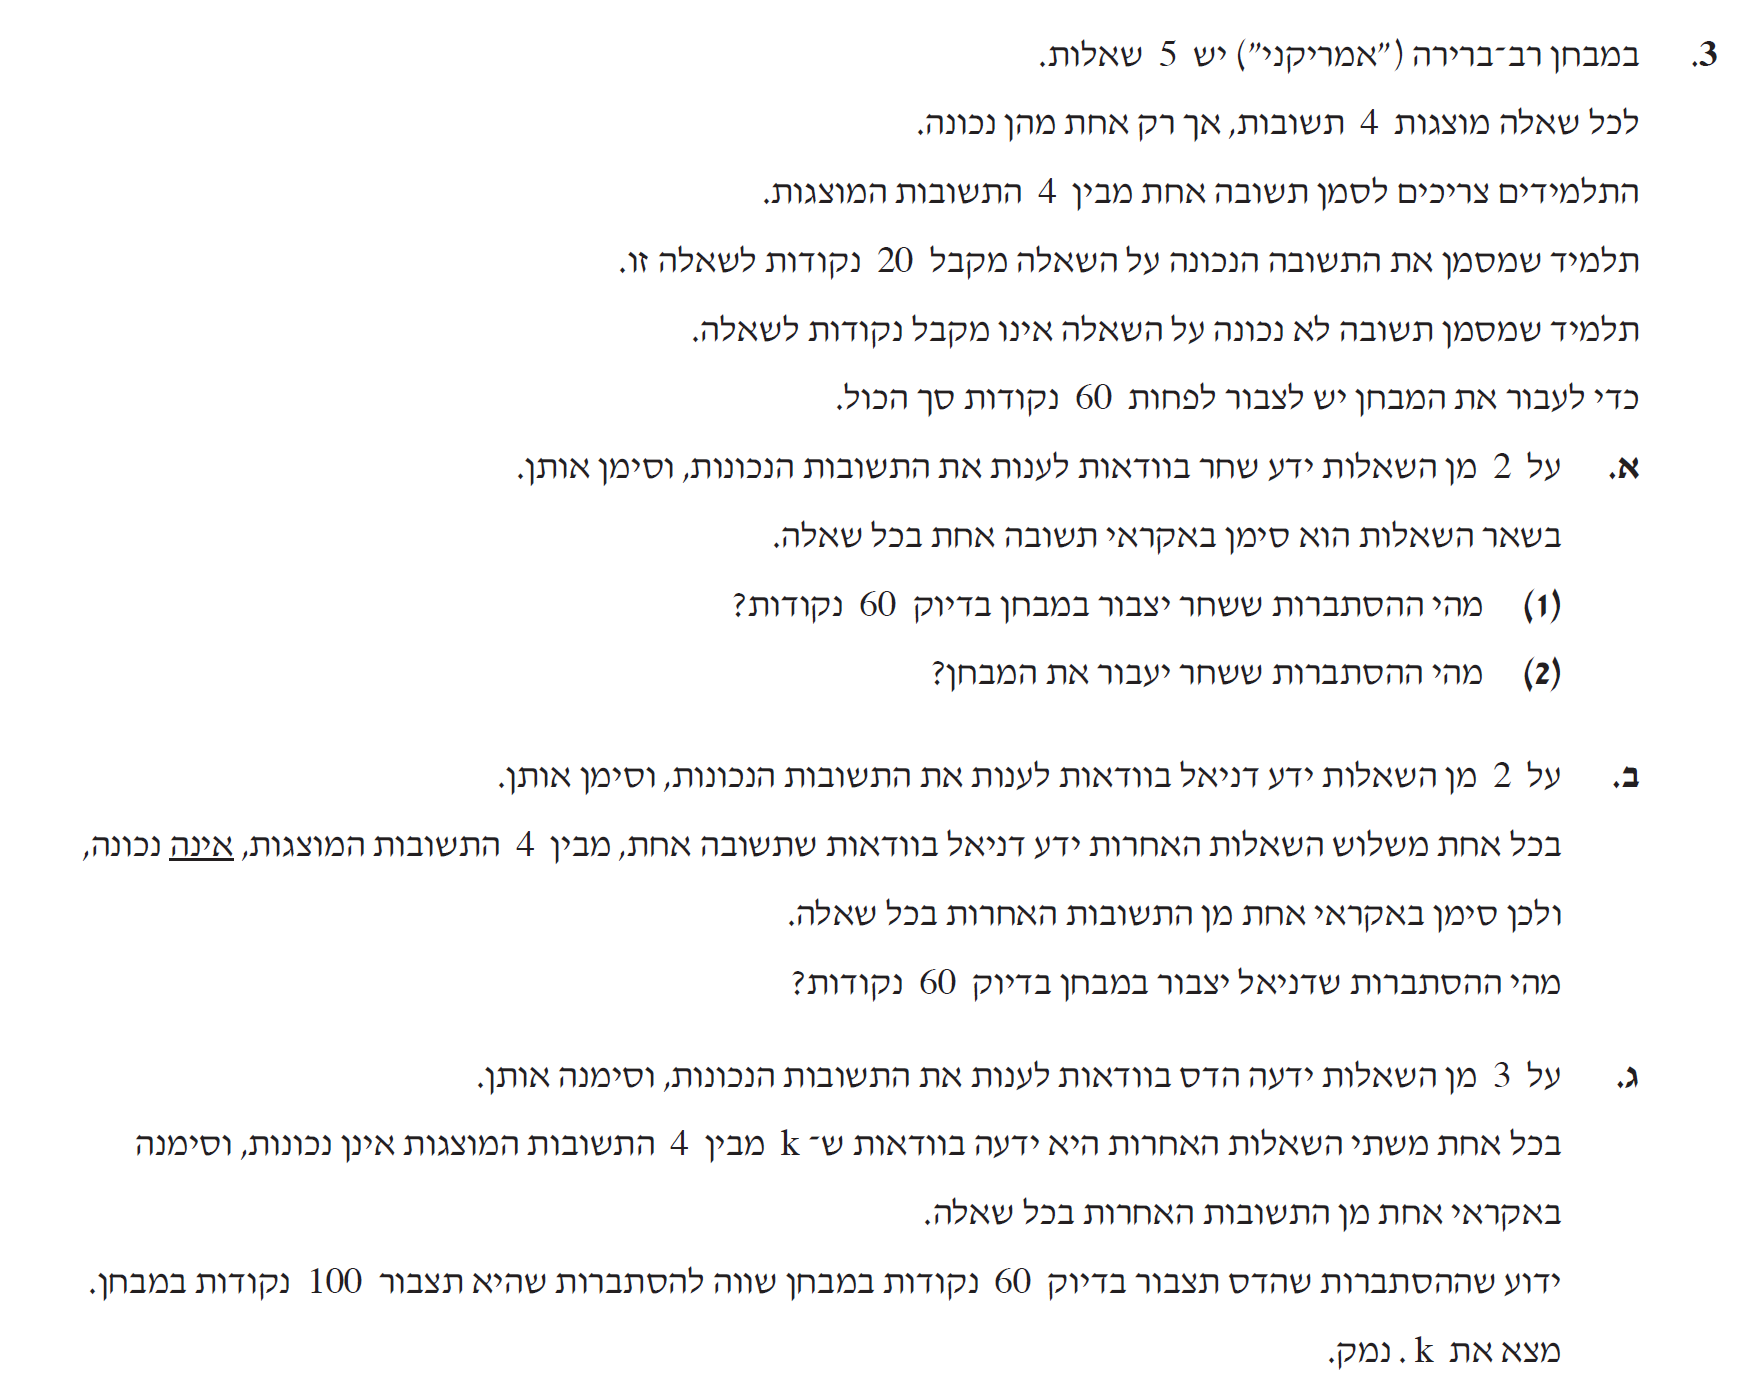
\includegraphics[width=\textwidth]{summer-2018b-3}
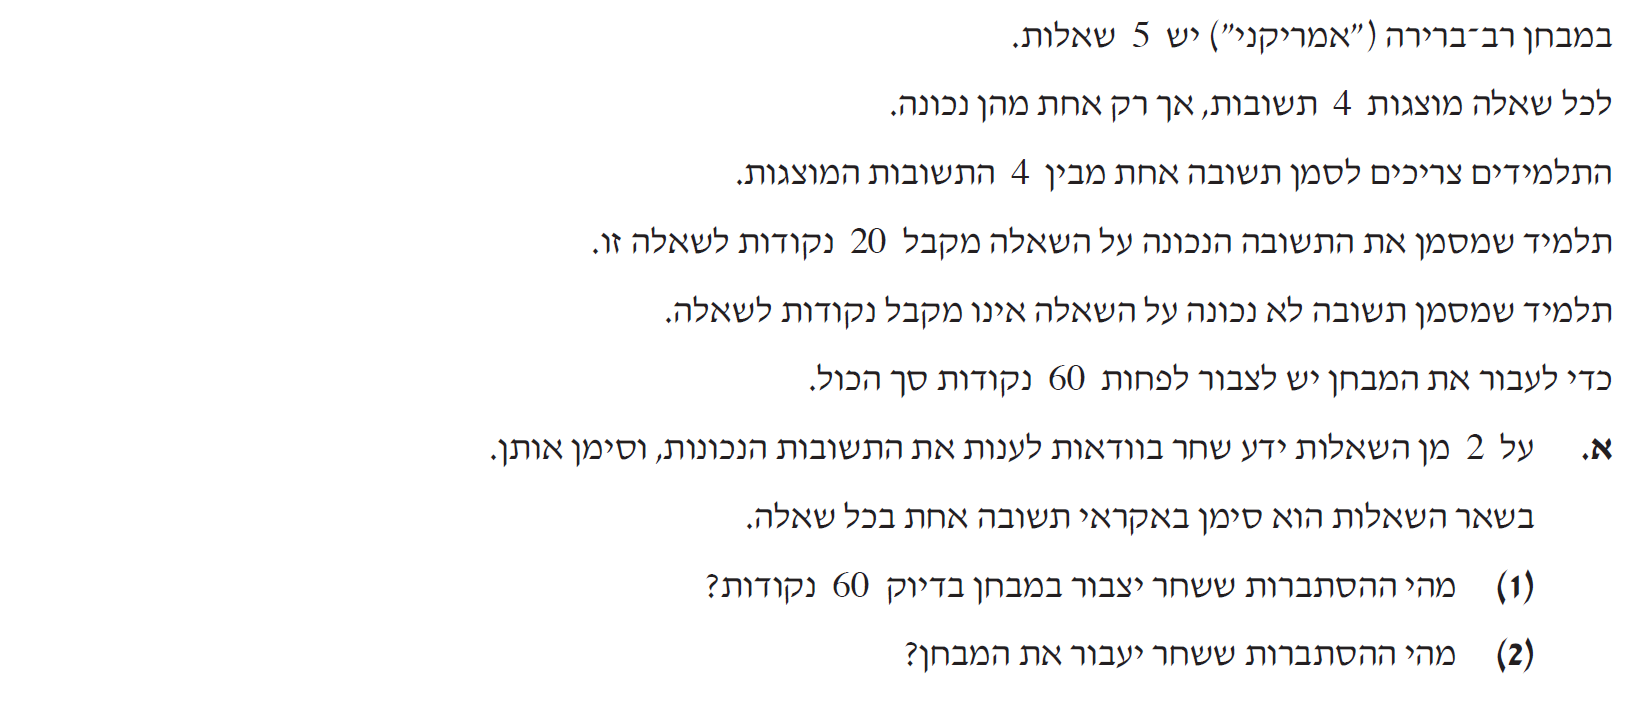
\includegraphics[width=\textwidth]{summer-2018b-3-1}
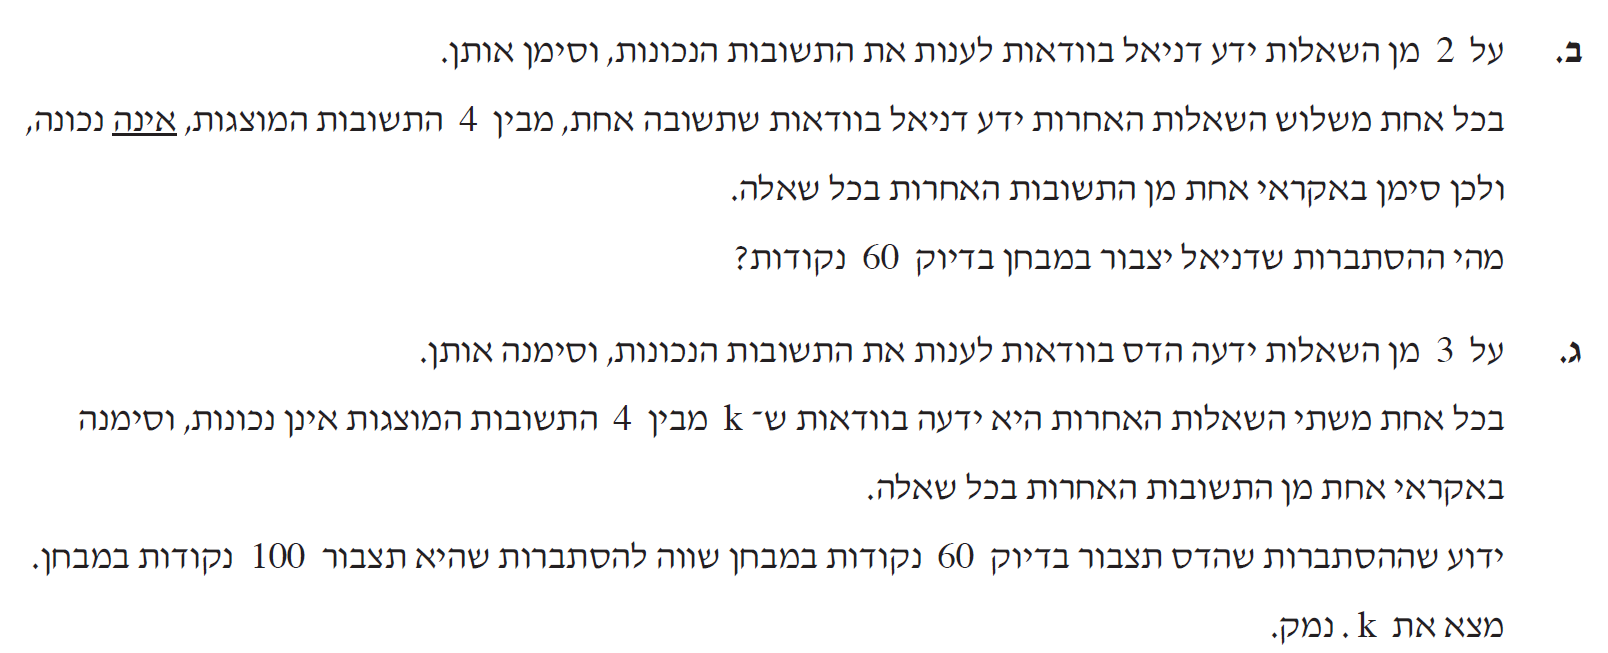
\includegraphics[width=\textwidth]{summer-2018b-3-2}
\end{center}

סעיף א
$(1)$.
שחר ידע שהוא ענה על שתי שאלות ולכן כדי לקבל ציון
$60$
עליו לענות על 
\textbf{בדיוק אחת}
משלושת השאלות האחרות, שניתן לחשב על ידי נוסחת ברנולי:
\[
{3 \choose 1}\left(\frac{1}{4}\right)\left(\frac{3}{4}\right)^2=\frac{27}{64}\,.
\]
סעיף א
$(2)$.
כדי לעבור את המבחן עליו לצבור
\textbf{לפחות}
שלוש תשובות נכונות. לכן, עלינה להוסיף את ההסבתרויות של ארבע וחמש תשובות נכונות:
\[
\frac{27}{64}+{3 \choose 2}\left(\frac{1}{4}\right)^2\left(\frac{3}{4}\right)^1+{3 \choose 3}\left(\frac{1}{4}\right)^3\left(\frac{3}{4}\right)^0=\frac{37}{64}\,.
\]
סעיף ב.
כמו שחר, דניאל צירך לענות נכון על שאלה אחת 
\textbf{בדיוק}
מתוך שלושת השאלות הנותרות. דניאל יודע שתשובה אחת מתוך ארבע לא נכונה, לכן ההסתברות שהוא יענה נכון על השאלה היא
$\frac{1}{3}$.
לפי נוסחת ברנולי:
\[
{3 \choose 1}\left(\frac{1}{3}\right)\left(\frac{2}{3}\right)^2=\frac{4}{9}\,.
\]
סעיף ג. אם הדס יודעת ש-%
$k$
מתוך 
$4$
תשובות לא נכונות, מספר התשובות שמהן היא בוחרת באקראי הוא
$4-k$.
הסיכוי לענות תשובה נכונה היא
$\frac{1}{4-k}$
וסיכוי לענות תשובה לא נכונה היא
$\frac{4-k-1}{4-k}$
כי אם תשובה אחת מתוך 
$4-k$,
נכונה כל שאר התשובות לא נכונות.

כדי לקבל ציון 
\textbf{בדיוק}
$100$
ברור שהדס צריכה לבחור תשובות נכונות לשתי השאלות הנותרות. כדי לקבל ציון 
\textbf{בדיוק}
$60$
עליה לבחר תשובות לא נכונות לשתי השאלות הנותרות. אין צורך להשתמש בנוסחת ברנולי במלואו:
\[
{n \choose k}p^k(1-p)^{n-k}\,,
\]
כי כאשר מחשבים את ההסתברות של "כל" או "אף אחד" הבחירה של 
$k$
מתוך
$n$
הוא אחד, כמו ההסתברות המשלימה לחזקת אפס. מספיק לחשב את ההסתברות של האירוע לחזקת מספר הסבבים:
\begin{eqnarray*}
\left(\frac{1}{4-k}\right)^2 &=&\left(\frac{4-k-1}{4-k}\right)^2\\
(3-k)^2&=&1\\
k^2-6k+8&=& 0\,.
\end{eqnarray*}
הפתרונות של המשוואה הם 
$k=2,k=4$
אבל נתון ש-"אחת מהן נכונה", לכן הפתרון האפשרי היחיד הוא
$k=2$.

%%%%%%%%%%%%%%%%%%%%%%%%%%%%%%%%%%%%%%%%%%%%%%%%%%%%%%%%%%%%%%%%%%%

\textbf{\R{
חורף תשע"ז
}}

\begin{center}
\selectlanguage{english}
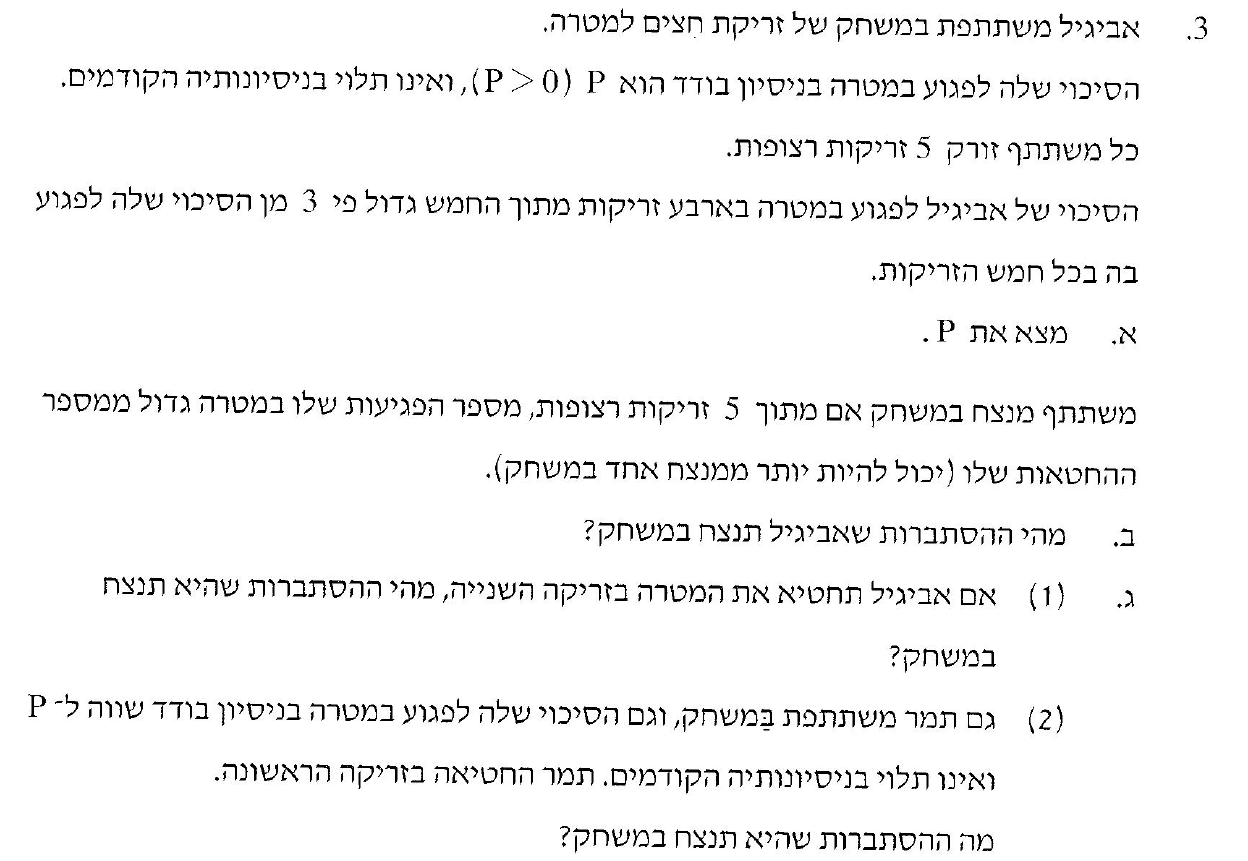
\includegraphics[width=.95\textwidth]{winter-2017-3.png}
\end{center}
\vspace{-1ex}

סעיף א. לפי נוסחת ברנולי:
\[
{5 \choose 4} p^4(1-p)^1 = 3{5\choose 5}p^5(1-p)^0\,.
\]
והפתרון הוא
$p=\frac{5}{8}$.

סעיף ב. ההסתברות ל-%
$3,4,5$
פגיעות היא:
\[
{5 \choose 3}p^3(1-p)^2 + {5 \choose 4}p^4(1-p)^1 + {5 \choose 5}p^5(1-p)^0
\]
נציב את
$p=\frac{5}{8}$
ונקבל
$0.7248$.

סעיף ג 
$(1)$.
מצאתי שניסוח השאלה לא בהיר. אני פירשתי אותה: מה ההסתברות של
\textbf{האירוע}
"אביגיל מחטיאה בזריקה השנייה ופוגעת בשלוש או ארבע מהזריקות האחרות"? כותב הבחינה התכוון להסתברות מותנת: "%
\textbf{אם ידוע ש-}%
אביגיל החטיאה בזריקה השנייה, מה ההסתברות שהיא פוגעת בשלוש או ארבע מהזריקות האחרות"?
\[
\renewcommand{\arraystretch}{2}
\begin{array}{c}
P(1,3,4,5\ \textrm{\R{אביגיל פגעה בשלוש או ארבע מהזריקות}}/\textrm{\R{אביגיל החטיאה בזריקה השניה}}) =\\
\displaystyle\frac{P(1,3,4,5\ \textrm{\R{אביגיל פגעה בשלוש או ארבע מהזריקות}}\cap \textrm{\R{אביגיל החטיאה בזריקה השניה}})}{P(\textrm{\R{אביגיל החטיאה בזריקה השניה}})}\,.
\end{array}
\]
אפשר לפתור את הבעיה בשתי דרכים. נתחיל עם הדרך הפשוטה יותר. נתון שהסיכוי לפגוע במטרה אינו תלוי בניסיונות הקודמים. לכן ההסתברויות בלתי תלויות והחישוב מצטמצם:

\[
\renewcommand{\arraystretch}{2}
\begin{array}{c}
\displaystyle\frac{P(1,3,4,5\ \textrm{\R{אביגיל פגעה בשלוש או ארבע מהזריקות}}) \cdot P(\textrm{\R{אביגיל החטיאה בזריקה השניה}})}{P(\textrm{\R{אביגיל החטיאה בזריקה השניה}})}\\
P(1,3,4,5\ \textrm{\R{אביגיל פגעה בשלוש או ארבע מהזריקות}})\,.
\end{array}
\]
החישוב הוא:
\[
{4\choose 4}\left(\frac{5}{8}\right)^4 \left(\frac{3}{6}\right)^0 +{4\choose 3}\left(\frac{5}{8}\right)^3\left(\frac{3}{8}\right)^1 = 0.5188\,.
\]
הדרך השנייה ארוכה יותר אבל מעניינת. האירוע של החיתוך בנוסחה להסתברות מותנית מורכבת משני אירועים. )א( לא משנה מה יצאה מהזריקה הראשונה, הזריקה השניה החטיאה, ושלושת הזריקות האחרונות פגעו. )ב( הזריקה הראשונה פגעה, הזריקה השניה החטיאה, ושתיים מתוך שלושת הזריקות האחרונות פגעו. נחשב את ההסתברות של האירועים האלה:
\[
1\cdot \frac{3}{8} \cdot \left(\frac{5}{8}\right)^3 \quad + \quad
\frac{5}{8}\cdot \frac{3}{8} \cdot \left[{3\choose 2}\left(\frac{5}{8}\right)^2\frac{3}{8}\right] = 0.1945\,.
\]
נחלק ב-%
$\frac{3}{8}$
ונקבל את התשובה 
$0.5188$.

סעיף ג 
$(2)$.
לא משנה איזו זריקה החטיאה, הזריקות בלתי תלויות וחישוב ההסתברות של "תמר פגעה בשלוש  או ארבע מהזריקות 
$2,3,4,5$"
נותן אותה תוצאה כמו האירוע "אביגיל פגעה בשלוש או ארבע מהזריקות 
$1,3,4,5$.

%%%%%%%%%%%%%%%%%%%%%%%%%%%%%%%%%%%%%%%%%%%%%%%%%%%%%%%%%%%%%%%%%%%
\bigskip

\textbf{\R{
קיץ תשע"ז, מועד א
}}

\begin{center}
\selectlanguage{english}
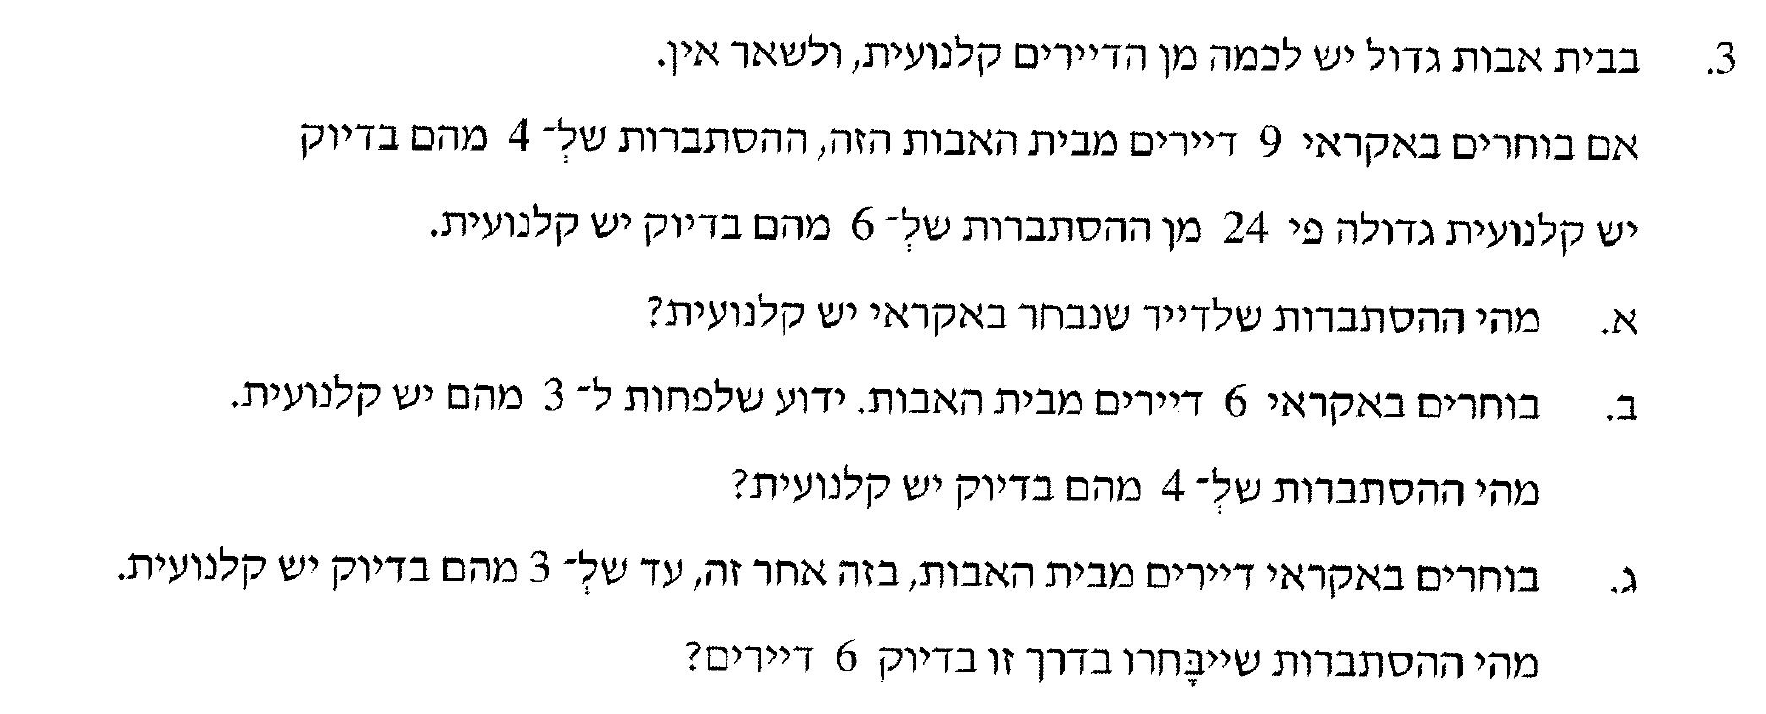
\includegraphics[width=.95\textwidth]{summer-2017a-3}
\end{center}

סעיף א. נסמן ב-%
$D$
את האירוע "דייר עם קלנועית" ואת ההסתברות של האירוע ב-%
$p$.
לפי נוסחת ברנולי:
\[
{9\choose 4} p^4 (1-p)^5=24 {9\choose 6} p^6 (1-p)^3\,.
\]
נפשט את המשוואה ונקבל משוואה ריבועית:
\[
15p^2+2p-1=0\,,
\]
עם שני פתרונות
$\frac{1}{5},-\frac{1}{3}$.
ההסתברות חייבת להיות חיובית ולכן התשובה היא 
$p=\frac{1}{5}=0.2$.

סעיף ב. המילה
\textbf{ידוע}
מכוונת אותנו להסתברות מותנת:
\[
P(D=4/D\ge3) = \frac{P(D=4\cap D\ge 3)}{P(D\ge 3)}\,.
\]
כאשר יש חפיפה בין ביטויים בחיתוך אפשר לפשט אותו. ברור שאם ערך גדול או שווה
$3$
\textbf{וגם}
שווה ל-%
$4$,
אז הוא שווה ל-%
$4$:
\[
P(D=4/D\ge3) =\frac{P(D=4)}{P(D\ge 3)}\,.
\]
לפי נוסחת ברנולי:
\[
P(D=4)={6\choose 4} 0.2^4 (1-0.2)^2= 0.01536\,.
\]
את הערך של
$P(D\ge 3)$
אפשר לחשב בשתי דרכים, בצורה ישירה או כאחד פחות המשלים:
\[
\renewcommand{\arraystretch}{1.4}
\begin{array}{l}
P(D\ge 3) = P(D=3) + P(D=4) + P(D=5) + P(D=6)\\
1- P(D<3)=1-(\,P(D=0) + P(D=1) + P(D=2)\,)\,.
\end{array}
\]
נבחר את האפשרות השנייה כי יש פחות גורמים בביטוי:
\[
1-0.2^0(1-0.2)^6-{6\choose 1}0.2^1(1-0.2)^5 - {6 \choose 2} 0.2^2(1-0.2)^4=0.099\,,
\]
והתשובה היא
$\displaystyle\frac{0.01536}{0.099}=0.15534$.

סעיף ג. הבחירה 
\textbf{האחרונה} 
תהיה "הצלחה" ויהיו שתי "הצלחות" בחמשת הבחירות הקודמות:
\[
\overbrace{\pm\;\pm\;\pm\;\pm\;\pm}^{2/5}\quad\quad \overbrace{+}^{1/1}\,.
\]
התשובה מתקבלת מנוסחת ברנולי לבחירות הראשונות כפול ההסתברות
$p$
לבחירה האחרונה:
\[
\left[{5\choose 2}0.2^2 (1-.02)^3\right]\cdot 0.2=0.04096\,.
\]

%%%%%%%%%%%%%%%%%%%%%%%%%%%%%%%%%%%%%%%%%%%%%%%%%%%%%%%%%%%%%%%%%%%

\textbf{\R{
קיץ תשע"ז, מועד ב
}}

\begin{center}
\selectlanguage{english}
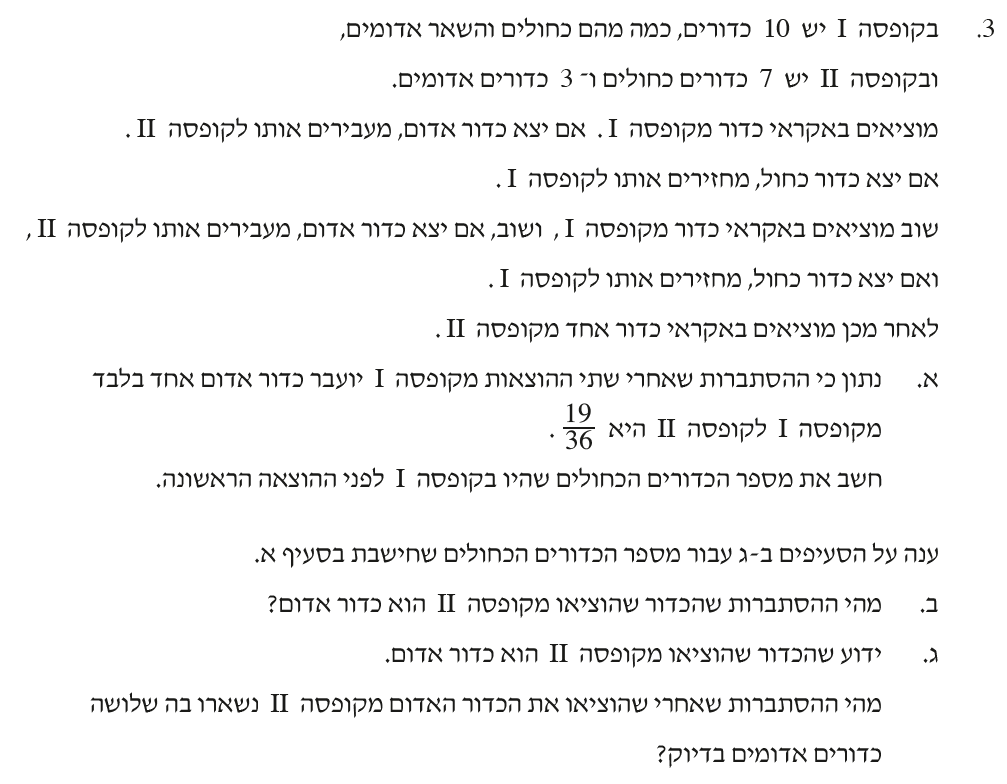
\includegraphics[width=.95\textwidth]{summer-2017b-3}
\end{center}

הביטוי
\textbf{מוציאים באקראי}
ואחר כך
\textbf{שוב מוציאים באקראי}
מכוון אותנו לשימוש בעץ כדי לתאר את הבחירה הסדרתית. נסמן ב-%
\textsf{A}
את מספר הכדורים האדומים בקופסה 
\textsf{I}.

באיור~%
\L{\ref{fig.summer-2017b.1}},
בכל צומת רשום שני זוגות של מספרים: מספר הכדורים האדומים ומספר הכדורים הכחולים בקופסה
\textsf{I},
ומתחתיו מספר הכדורים האדומים ומספר הכדורים הכחולים בקופסה
\textsf{II}.
הכוכבית מסמנת את שתי האפשרויות בהן הוצאנו כדור אדום אחד בדיוק מקופסה
\textsf{I}.
שימו לב שמספר הכדורים הכחולים בכל אחת המקופסאות לא משתנה.
\begin{figure}
\begin{center}
\selectlanguage{english}
\begin{tikzpicture}
[grow=right,
level 1/.append style={font=\sffamily,text width=2cm,level distance=3.5cm,sibling distance=10em},
level 2/.append style={font=\sffamily,text width=2.5cm,level distance=4.5cm,sibling distance=5em}]
\node[font=\sffamily,text width=2cm] {(A,10-A)\\(3,7)} % root
child {
  node {(A,10-A)\\(3,7)}
    child {
      node {(A,10-A)\\(3,7)}
      edge from parent node[below] {\R{כחול} I}
    }
    child {
      node {(A-1,10-A)\ *\\(4,7)}
      edge from parent node[above] {\R{אדום} I}
    }
    edge from parent node[below] {\R{כחול} I}
}
child { 
  node {(A-1,10-A)\\(4,7)}
    child {
      node {(A-1,10-A)\ *\\(4,7)}
      edge from parent node[below] {\R{כחול} I}
    }
    child {
      node {(A-2,10-A)\\(5,7)}
      edge from parent node[above] {\R{אדום} I}
    }
    edge from parent node[above] {\R{אדום} I}
};
\end{tikzpicture}
\selectlanguage{hebrew}
\caption{עץ ההסתברויות של הוצאת הכדורים}\label{fig.summer-2017b.1}
\end{center}
\end{figure}
נשווה את הסתברות הנתונה לשתי האפשרויות לסכום ההסתברויות של שני המסלולים:
\[
\frac{A}{10}\cdot\frac{10-A}{9} + \frac{10-A}{10}\cdot\frac{A}{10} = \frac{19}{36}\,.
\]
נפשט ונקבל משוואה ריבועית 
$x^2-10a+25=0$
שיש לה פתרון אחד
$a=$,
שהוא גם מספר הכדורים הכחולים  וגם מספר הכדורים האדומים בקופסה
\textsf{I}.

סעיף ב. עבור כל מצב סופי, ההסתברות להוציא כדור אדום מקופסה
\textsf{II}
הוא מספר הכדורים האדומים בקופסה לחלק למספר הכדורים בקופסה:
\[
\frac{5}{5+7},\; \frac{4}{4+7},\; \frac{4}{4+7},\; \frac{3}{3+7}\,.
\]
כדי לקבל את ההסתברות לכל המצבים, נסכם את ההסתברויות אלו לאחר הכפלתן בהסתברות להגיע למצב:
\[
\frac{5}{10}\cdot\frac{4}{9}\cdot\frac{5}{12}+\frac{5}{10}\cdot\frac{5}{9}\cdot\frac{4}{11}+\frac{5}{10}\cdot\frac{5}{10}\cdot\frac{4}{11}+\frac{5}{10}\cdot\frac{5}{10}\cdot\frac{3}{10}=0.3595\,.
\]

סעיף ג. המילה 
\textbf{ידוע}
מכוון להסתברות מותנת. אם רואים באיור שיישארו שלושה כדורים אדומים רק אם היו אברעה כדורים אדומים לפני הבחירה, כלומר, אותם שני מצבים המסומנים כוכבית.
\[
\begin{array}{c}
P(\textrm{II \R{נשארו שלושה אדומים בקופסה}}/\textrm{II \R{הוציאו כדור אדום מקופסה}}) =\\\\
\displaystyle\frac{P(\textrm{II \R{נשארו שלושה אדומים בקופסה}} \cap \textrm{II \R{הוציאו כדיר אדום מקופסה}})}{P(\textrm{II \R{הוציאו כדור אדום מקופסה}})}
\end{array}
\]
ההסדברות במנה היא ההסתברות )הנתונה!( שנגיע לאחד המצבים המסומנים בכוכבית כפול ההסתברות לבחור אדום מקופסה 
\textsf{II},
וההסתברות במכנה חישבנו בסעיף ב. התשובה היא:
\[
\frac{\displaystyle\frac{19}{36}\cdot\frac{4}{11}}{0.3595}=0.53385\,.
\]

%%%%%%%%%%%%%%%%%%%%%%%%%%%%%%%%%%%%%%%%%%%%%%%%%%%%%%%%%%%%%%%%%%%

\textbf{\R{
חורף תשע"ו
}}

\begin{center}
\selectlanguage{english}
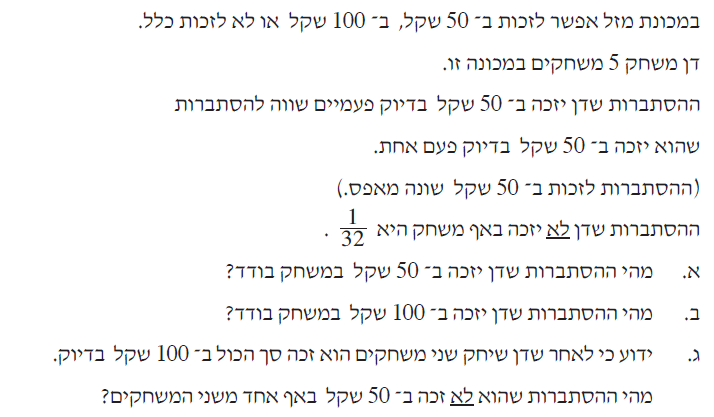
\includegraphics[width=.95\textwidth]{winter-2016-3}
\end{center}
נתון שיש שלוש אפשרויות עבור זכיה במשחק ולכן יש שלוש הסתברויות שסכומן אחד:
\[
P(0) + P(50) + P(100) = 1\,.
\]
סעיף א. ההסתברות שדן לא זכה באף אחד מחמישה משחקים היא 
$P(0)^5$.
נתון שהערך הזה הוא 
$\frac{1}{32}$,
ולכן 
$P(0)=\frac{1}{2}$.
לפי המידע הנתון:
\begin{eqnarray*}
{5\choose 2} P(50)^2 (1-P(50))^3 &=& {5\choose 1} P(50) (1-P(50))^4\\
P(50)&=&\frac{1}{3}\,.
\end{eqnarray*}
סעיף ב. מייד מתקבל
$P(100) = 1 - P(0) - P(50) = 1-\frac{1}{2}-\frac{1}{3}=\frac{1}{6}$.

סעיף ג. 
\textbf{ידוע כי}
מכוון להסתברות מותנת:
\[
\begin{array}{c}
P(\textrm{\R{ באף משחק}}50\textrm{\R{לא זכה ב-}}
/
100\textrm{\R{זכה ב-}}) =\\\\
\displaystyle\frac{
P(\textrm{\R{ באף משחק}}50\textrm{\R{לא זכה ב-}}
\cap
100\textrm{\R{זכה ב-}})
}
{P(100\textrm{\R{זכה ב-}})}\,.
\end{array}
\]
נתבונן בעץ המציג את תוצאות שני המשחקים )איור~%
\L{\ref{fig.winter-2017.1}}(.
הסימן
$=$
מסמן שדן זכה ב-%
$100$,
והסימן
$\neq$
מסמן שדן לא זכה ב-%
$50$
באף אחד משני המשחקים.
\begin{figure}
\begin{center}
\selectlanguage{english}
\begin{tikzpicture}
[grow=right,
level 1/.append style={font=\sffamily,level distance=3cm,sibling distance=8em},
level 2/.append style={font=\sffamily,level distance=4cm,sibling distance=3em}]
\node[left] {$0$} % root
child {
  node[right] {$100$}
    child {
      node[right] {$200\quad \neq$}
      edge from parent node[below] {$\frac{1}{6}$}
    }
    child {
      node[right] {$150$}
      edge from parent node[below,xshift=2em] {$\frac{1}{3}$}
    }
    child {
      node[right] {$100\quad =\quad \neq$}
      edge from parent node[above] {$\frac{1}{2}$}
    }
    edge from parent node[below] {$\frac{1}{6}$}
}
child {
  node[right] {$50$}
    child {
      node[right] {$150$}
      edge from parent node[below] {$\frac{1}{6}$}
    }
    child {
      node[right] {$100\quad =$}
      edge from parent node[below,xshift=2em] {$\frac{1}{3}$}
    }
    child {
      node[right] {$50$}
      edge from parent node[above] {$\frac{1}{2}$}
    }
    edge from parent node[below] {$\frac{1}{3}$}
}
child {
  node[right] {$0$}
    child {
      node[right] {$100\quad =\quad \neq$}
      edge from parent node[below] {$\frac{1}{6}$}
    }
    child {
      node[right] {$50$}
      edge from parent node[below,xshift=2em] {$\frac{1}{3}$}
    }
    child {
      node[right] {$0\quad \neq$}
      edge from parent node[above] {$\frac{1}{2}$}
    }
    edge from parent node[above] {$\frac{1}{2}$}
}
;
\end{tikzpicture}
\selectlanguage{hebrew}
\caption{עץ ההסתברויות של המשחקים}\label{fig.winter-2017.1}
\end{center}
\end{figure}
חישוב ההסתברות המותנת:
\[
\frac{\displaystyle\frac{1}{2}\cdot\frac{1}{6} + \frac{1}{6}\cdot \frac{1}{2}}{\displaystyle\frac{1}{2}\cdot\frac{1}{6} + \frac{1}{3}\cdot \frac{1}{3}+ \frac{1}{6}\cdot \frac{1}{2}}  =  \frac{\displaystyle\frac{1}{6}}{\displaystyle\frac{5}{18}}=\frac{3}{5}\,.
\]

%%%%%%%%%%%%%%%%%%%%%%%%%%%%%%%%%%%%%%%%%%%%%%%%%%%%%%%%%%%%%%%%%%%

\textbf{\R{
קיץ תשע"ו, מועד א
}}

\begin{center}
\selectlanguage{english}
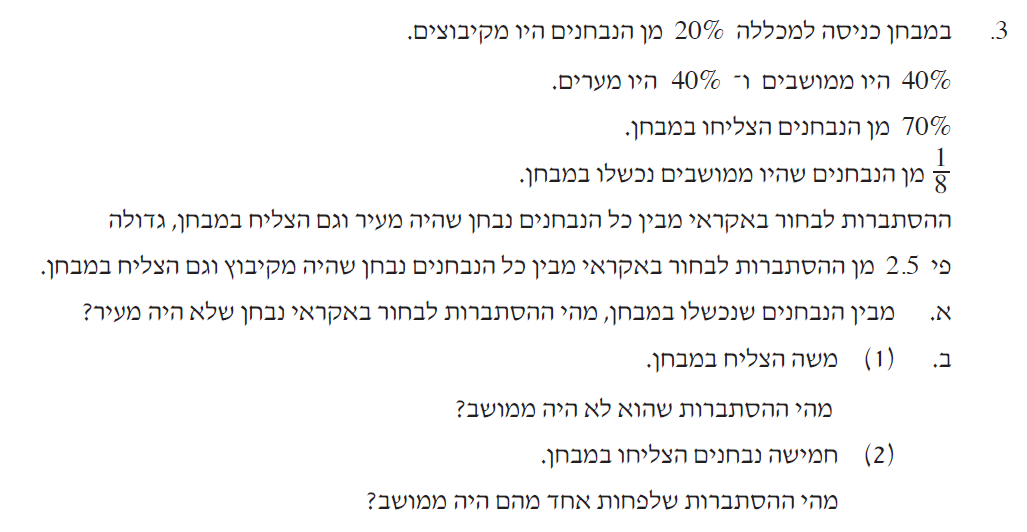
\includegraphics[width=\textwidth]{summer-2016a-3}
\end{center}

נסמן 
$=S$
נבחנים שהצליחו,
$=K$
נבחנים מקיבוצים,
$=M$
נבחנים ממושבים,
$=E$
נבחנים מערים,
$p=P(K\cap S$,
ההסתברות שנבחנים מקיבוצים הצליחו במבחן. ההסתברויות
$P(K),P(M),P(E)$
נתונות, כמו גם ההסתברות של
$P(S)$,
ולכן 
$P(\overline{S})=1-P(S)$.
לבסוף, נתונה ההסתברות
$P(M\cap \overline{S})$,
והיחס
$P(E\cap S)=2.5P(K\cap S)$.
נסכם את המידע הנתונה בטבלה:
\begin{center}
\selectlanguage{english}
\begin{tikzpicture}[scale=1.25]
\draw (0,0) grid (4,3);
\node at (3.5,3.3) {$\bm{K}$};
\node at (2.5,3.3) {$\bm{M}$};
\node at (1.5,3.3) {$\bm{E}$};
\node at (4.3,2.5) {$\bm{S}$};
\node at (4.3,1.5) {$\bover{S}$};

\node at (0.5,2.5) {$0.70$};
\node at (0.5,1.5) {$0.30$};
\node at (0.5,0.5) {$1.0$};

\node at (1.5,2.5) {$2.5p$};
%\node at (1.5,1.5) {$$};
\node at (1.5,0.5) {$0.40$};

\node at (2.5,2.5) {$0.35$};
\node at (2.5,1.5) {$0.05$};
\node at (2.5,0.5) {$0.40$};

\node at (3.5,2.5) {$p$};
%\node at (3.5,1.5) {$$};
\node at (3.5,0.5) {$0.20$};
\end{tikzpicture}
\end{center}
נכתוב את המידע בשורה עבור
$S$
כמשוואה:
\begin{eqnarray*}
p+0.35+2.5p&=&0.70\\
p&=&0.1\,.
\end{eqnarray*}
כעת ניתן למלא את הטבלה:
\begin{center}
\selectlanguage{english}
\begin{tikzpicture}[scale=1.25]
\draw (0,0) grid (4,3);
\node at (3.5,3.3) {$\bm{K}$};
\node at (2.5,3.3) {$\bm{M}$};
\node at (1.5,3.3) {$\bm{E}$};
\node at (4.3,2.5) {$\bm{S}$};
\node at (4.3,1.5) {$\bover{S}$};

\node at (0.5,2.5) {$0.70$};
\node at (0.5,1.5) {$0.30$};
\node at (0.5,0.5) {$1.0$};

\node at (1.5,2.5) {$0.25$};
\node at (1.5,1.5) {$0.15$};
\node at (1.5,0.5) {$0.40$};

\node at (2.5,2.5) {$0.35$};
\node at (2.5,1.5) {$0.05$};
\node at (2.5,0.5) {$0.40$};

\node at (3.5,2.5) {$0.10$};
\node at (3.5,1.5) {$0.10$};
\node at (3.5,0.5) {$0.20$};
\end{tikzpicture}
\end{center}
סעיף א. לפי הנוסחה להסתברות מותנת:
\[
P(\overline{E}/\overline{S})=P((K\cup M)/\overline{S}) = \frac{P(K\cap \overline{S})+P(M\cap \overline{S})}{P(\overline{S})}=\frac{0.10+0.05}{0.30}=\frac{1}{2}\,.
\]
סעיף ב
$(1)$.
לפי הנוסחה להסתברות מותנת:
\[
P(\overline{M}/S)=P((K\cup E)/S) = \frac{P(K\cap S)+P(E\cap S)}{P(S)}=\frac{0.10+0.25}{0.70}=\frac{1}{2}\,.
\]
סעיף ב
$(2)$.
%את ההסתברות שנבחן שהצליח המושב ניתן לחשב בדיוק כמו בסעיף ב
%$(1)$,
%אבל ההסתברות זו היא המשלים של ההסתברות שחושב שם
%$P(M/S)=1-P(\overline{M}/S)=1-\frac{1}{2}=\frac{1}{2}$.
"לפחות אחד ממושב" הוא המשלים ל-"כולם לא מהמושב":
\[
1-P(\overline{M}/S)^5=1-\left(\frac{1}{2}\right)^2=\frac{31}{32}\,.
\]
%%%%%%%%%%%%%%%%%%%%%%%%%%%%%%%%%%%%%%%%%%%%%%%%%%%%%%%%%%%%%%%%%%%

\textbf{\R{
קיץ תשע"ו, מועד ב
}}

\begin{center}
\selectlanguage{english}
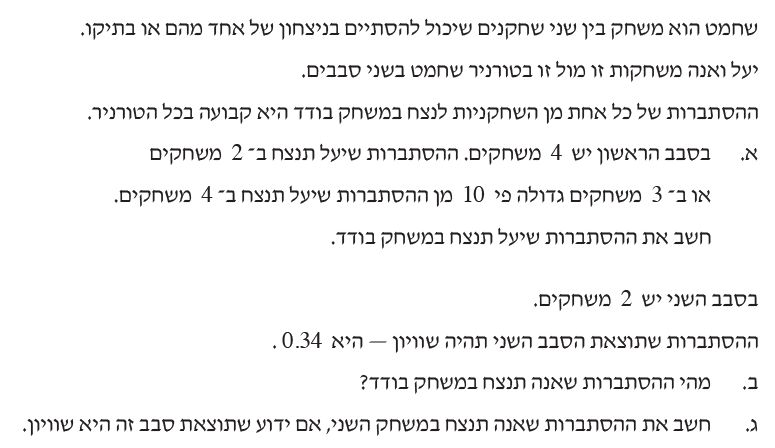
\includegraphics[width=\textwidth]{summer-2016b-3}
\end{center}
נסמן:
$=y$
ההסתברות שיעל תנצח במשחק בודד, 
$=a$
ההסתברות שאנה תנצח במשחק בודד.

סעיף א. בדרך כלל כאשר כותבים
\textbf{גדולה פי} $n$,
ההשוואה היא בין שני אירועים. שימו לב שבסעיף זה רק יעל מופיעה. לפי נוסחת ברנולי:
\[
{4 \choose 2}y^2(1-y)^2 + {4\choose 3}y^3(1-y) = 10\cdot {4\choose 4}y^4(1-y)^0\,.
\]
נפשט ונקבל משוואה ריבועית
$4y^2+4y-3=0$
שהשורש החיובי היחיד שלה היא
$y=\frac{1}{2}$.

סעיף ב. כדאי לצייר עץ של האירועים, אבל אוותר עליו בסעיף זה. האפשרויות לקבל שוויון הן ניצחון אחד לאנה וליעל או תיקן בשני המשחקים. ההסתברות לתיקו היא המשלים לסכום ההסתברויות שאחת מהן תנצח. חישבנו בסעיף א את ההסתברות שיעל תנצח ולכן מקבלים משוואה בנעלם הבודד שאנה תנצח:
\begin{eqnarray*}
{2 \choose 1}ya + (1-(y+a))^2 &=& 0.34\\
2\cdot \frac{1}{2}\cdot a + (\frac{1}{2}-a)^2&=&0.34\\
a&=&0.3\,.
\end{eqnarray*}

סעיף ג. המילים
\textbf{אם ידוע}
מכוונות להסתברות מותנית"
\[
\begin{array}{c}
P(\textrm{\R{אנה תנצח במשחק השני}} / \textrm{\R{תוצאת הסבב היא שוויון}})=\\\\
\displaystyle\frac{
P(\textrm{\R{אנה תנצח במשחק השני}} \cap \textrm{\R{תוצאת הסבב היא שוויון}})
}
{P(\textrm{\R{תוצאת הסבב היא שוויון}})}\,.
\end{array}
\]
ההסתברות לשיוון בסבב נתונה ואם אנה תנצח בסבב עם שיוויון זה רק אם גם יעל תנצח:
\[
P(\textrm{\R{אנה תנצח במשחק השני}} / \textrm{\R{תוצאת הסבב היא שוויון}})= \frac{ya}{.34}=\frac{\displaystyle\frac{.3}{2}}{.34}=0.4412\,.
\]

%%%%%%%%%%%%%%%%%%%%%%%%%%%%%%%%%%%%%%%%%%%%%%%%%%%%%%%%%%%%%%%%%%%
\newpage

\textbf{\R{
חורף תשע"ה
}}

\begin{center}
\selectlanguage{english}
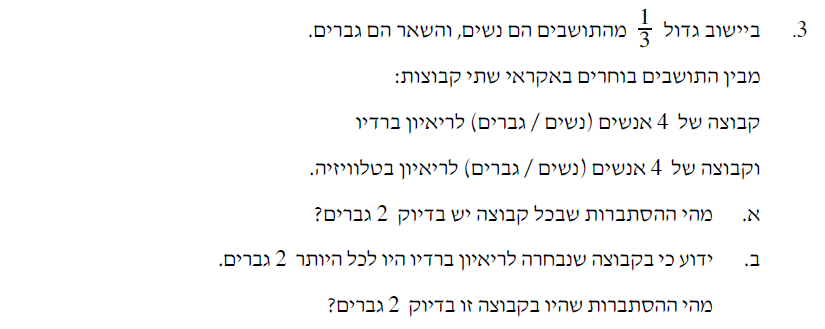
\includegraphics[width=\textwidth]{winter-2015-3}
\end{center}

"יישוב גדול" אומר לי שניתן לבחור מספר רב של תושבים, לפחות שמונה אנשים כפי שנדרש.

סעיף א. כל קבוצה היא בחירה בלתי תלוייה שנחשב לפי נוסחת ברנולי:
\[
{4 \choose 2}\left(\frac{2}{3}\right)^2\left(\frac{1}{3}\right)^2=\frac{8}{27}\,.
\]
כדי לקבל את ההסתברות שלשתי הקבוצות יהיו בדיוק שני גברים, נעלה ערך זה בריבוע:
\[
\left(\frac{8}{27}\right)^2=\frac{64}{729}\,.
\]

סעיף ב. המילים
\textbf{ידוע ש} 
מכוונות להסתברות מותנית:
\[
\begin{array}{c}
P(\textrm{\R{בדיוק שני גברים}} / \textrm{\R{לכל היותר שני גברים}})=\\\\
\displaystyle\frac{
P(\textrm{\R{בדיוק שני גברים}} \cap \textrm{\R{לכל היותר שני גברים}})
}
{P(\textrm{\R{לכל היותר שני גברים}})}\,.
\end{array}
\]
שימו לב שהחיתוך במנה שקולה ל-"בדיוק שני גברים" כי המשמעות של "לכל היותר שני גברים" היא 
$0,1,2$
גברים. ערך זה חישבנו בסעיף הקודם. "לכל היותר שני גברים" הוא הסכום של שלוש נוסחאות ברנולי:
\[
\left(\frac{2}{3}\right)^0\left(\frac{1}{3}\right)^4 + {4\choose 1}\left(\frac{2}{3}\right)^1\left(\frac{1}{3}\right)^3 + {4\choose 2}\left(\frac{2}{3}\right)^2\left(\frac{1}{3}\right)^2=\frac{11}{27}\,
\]
והתשובה לשאלה היא:
\[
\frac{8/27}{11/27}=\frac{8}{11}\,.
\]

%%%%%%%%%%%%%%%%%%%%%%%%%%%%%%%%%%%%%%%%%%%%%%%%%%%%%%%%%%%%%%%%%%%

\textbf{\R{
קיץ תשע"ה, מועד א
}}

\begin{center}
\selectlanguage{english}
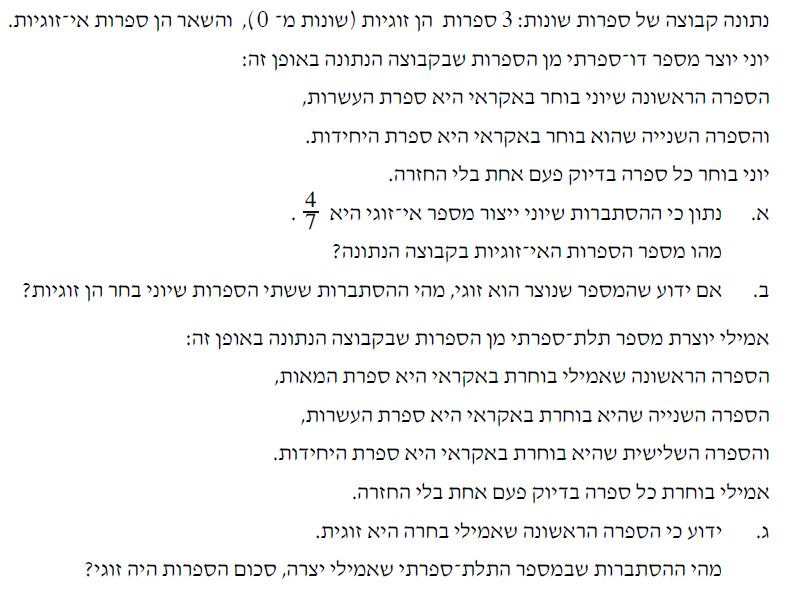
\includegraphics[width=\textwidth]{summer-2015a-3}
\end{center}

השאלה ארוכה וחובה לקרוא אותה בעיון. נסמן 
$=n$
מספר הספרות בקבוצה, כך שמספר הזוגיים הוא 
$3$
ומספר האי-זוגיים הוא
$n-3$.
השאלה מתארת בחירה של "הספרה הראשונה" ואחר כך "הספרה הראשונה", תיאור המכוון לעץ הסתברויות )איור~%
\L{\ref{fig.summer-2015a.1}}(.

\begin{figure}[bt]
\begin{center}
\selectlanguage{english}
\begin{tikzpicture}
[grow=right,
level 1/.append style={text width=2cm,level distance=3.5cm,sibling distance=8em},
level 2/.append style={text width=2.5cm,level distance=4.5cm,sibling distance=4em}]
\node[text width=2cm] {$\left(\frac{3}{n},\frac{n-3}{n}\right)$} % root
child {
  node {$\left(\frac{3}{n-1},\frac{n-4}{n-1}\right)$}
    child {
      node {$\left(\frac{3}{n-2},\frac{n-5}{n-2}\right)\quad *$}
      edge from parent node[below,xshift=5mm,yshift=-1mm] {\R{אי-זוגי}}
    }
    child {
      node {$\left(\frac{2}{n-2},\frac{n-4}{n-2}\right)$}
      edge from parent node[above,xshift=5mm,yshift=1mm] {\R{זוגי}}
    }
    edge from parent node[below,yshift=-1mm] {\R{אי-זוגי}}
}
child { 
  node {$\left(\frac{2}{n-1},\frac{n-3}{n-1}\right)$}
    child {
      node {$\left(\frac{2}{n-2},\frac{n-4}{n-2}\right)\quad *$}
      edge from parent node[below,xshift=5mm,yshift=-1mm] {\R{אי-זוגי}}
    }
    child {
      node {$\left(\frac{1}{n-2},\frac{n-3}{n-2}\right)$}
      edge from parent node[above,xshift=5mm,yshift=1mm] {\R{זוגי}}
    }
    edge from parent node[above] {\R{זוגי}}
};
\end{tikzpicture}
\selectlanguage{hebrew}
\caption{עץ ההסתברויות של בחירת הספרות}\label{fig.summer-2015a.1}
\end{center}
\end{figure}

סעיף א. המספר יהיה אי-זוגי אם 
\textbf{הבחירה השנייה}
תהיה של ספרה אי-זוגית. המסלולים האלה מסומנים בכוכבית באיור. נשווה את סכום ההסתברויות של המסלולים לערך הנתון:
\[
\frac{3}{n}\cdot\frac{n-3}{n-1} + \frac{n-3}{n}\cdot\frac{n-4}{n-1} = \frac{4}{7}\,.
\]
נפשט את משוואה ונקבל משוואה ריבועית
$n^2-8n+7=0$
שיש לה שני פתרונות לא-שליליים
$n=1,n=7$.
נתון שיש לפחות שלוש ספרות, לכן מספר הספרות הוא
$7$.
נשים לב שהשאלה מבקשת את מספר הספרות 
\textbf{האי-זויות}
ולכן התשובה היא
$7-3=4$.

סעיף ב. המילים 
\textbf{אם ידוע}
מכוונות להסתברות מותנית. אם המספר שנוצר זוגי, הספרה האחרונה היא זוגית:
\[
\begin{array}{c}
P(\textrm{\R{שתי ספרות זוגיות}} / \textrm{\R{ספרה אחרונה זוגית}})=\\\\
\displaystyle\frac{
P(\textrm{\R{שתי ספרות זוגיות}} \cap \textrm{\R{ספרה אחרונה זוגית}})
}
{P(\textrm{\R{ספרה אחרונה זוגית}})}=\\\\
\displaystyle\frac{
P(\textrm{\R{שתי ספרות זוגיות}})
}
{P(\textrm{\R{ספרה אחרונה זוגית}})}\,.
\end{array}
\]
את החיתוך אפשר לפשט כי אם שתי הספרות זוגיות, הספרה האחרונה חייבת להיות זוגית.

ניתן לחשב את ההסתברות "ספרה אחרונה זוגית" לפי המידע בעץ ההסתברויות או פשוט לשים לב שהיא המשלימה לערך הנתון בסעיף א של "הספרה האחרונה אי-זוגית". נחשב את ההסתברות במנה לפי המסלול הבודד בעץ ההסתברויות )איור~
\L{\ref{fig.summer-2015a.2}}(
של בחירה של שתי ספרות זוגיות:
\[
\frac{\displaystyle\frac{3}{7}\cdot\frac{2}{6}}{1-\displaystyle\frac{4}{7}}=\frac{1}{3}\,.
\]

\begin{figure}
\begin{center}
\selectlanguage{english}
\begin{tikzpicture}
[grow=right,
level 1/.append style={level distance=3cm,sibling distance=8em},
level 2/.append style={level distance=4cm,sibling distance=4em}]
\node {$\left(\frac{3}{7},\frac{4}{7}\right)$} % root
child {
  node {$\left(\frac{3}{6},\frac{3}{6}\right)$}
    child {
      node {$\left(\frac{3}{5},\frac{2}{5}\right)$}
      edge from parent node[below,xshift=5mm,yshift=-3mm] {\R{אי-זוגי}}
    }
    child {
      node {$\left(\frac{2}{5},\frac{3}{5}\right)$}
      edge from parent node[above,xshift=5mm,yshift=1mm] {\R{זוגי}}
    }
    edge from parent node[below,yshift=-3mm] {\R{אי-זוגי}}
}
child { 
  node {$\left(\frac{2}{6},\frac{4}{6}\right)$}
    child {
      node {$\left(\frac{2}{5},\frac{3}{5}\right)$}
      edge from parent node[below,xshift=5mm,yshift=-3mm] {\R{אי-זוגי}}
    }
    child {
      node {$\left(\frac{1}{5},\frac{4}{5}\right)$}
      edge from parent node[above,xshift=5mm,yshift=1mm] {\R{זוגי}}
    }
    edge from parent node[above,yshift=2mm] {\R{זוגי}}
};
\end{tikzpicture}
\selectlanguage{hebrew}
\caption{עץ ההסתברויות של בחירת הספרות}\label{fig.summer-2015a.2}
\end{center}
\end{figure}

סעיף ג. הסכום יהיה זוגי רק אם שתי הספרות האחרונת הן זוגיות או אי-זוגיות:
\begin{eqnarray*}
2k_1+2k_2+2k_3&=&2(k_1+k_2+k_3)\\
2k_1+2(k_2+1)+2(k_3+1)&=&2(k_1+k_2+k_3+1)\,.
\end{eqnarray*}
גם סעיף זה עוסק בהסתברות מותנית, אבל כאן שתי ההסתברויות בלתי תלויות )בחירה הספרה הראשונה לא משפיע על בחירת שתי הספרות האחרות(, לכן אפשר לבטא את החיתוך כמכפלה והחישוב מצטמצם:
\[
\begin{array}{c}
P(\textrm{\R{סכום זוגי}} / \textrm{\R{ספרה ראשונה זוגית}})=\\\\
\displaystyle\frac{
P(\textrm{\R{סכום זוגי}} \cap \textrm{\R{ספרה ראשונה זוגית}})
}
{P(\textrm{\R{ספרה ראשונה זוגית}})}=\\\\
\displaystyle\frac{
P(\textrm{\R{סכום זוגי}}) \cdot P(\textrm{\R{ספרה ראשונה זוגית}})
}
{P(\textrm{\R{ספרה ראשונה זוגית}})}=\\\\
P(\textrm{\R{סכום זוגי}})\,.
\end{array}
\]

\begin{figure}
\begin{center}
\selectlanguage{english}
\begin{tikzpicture}
[grow=right,
level 1/.append style={level distance=3cm,sibling distance=8em},
level 2/.append style={level distance=4cm,sibling distance=4em}]
\node {$\left(\frac{2}{6},\frac{4}{6}\right)$} % root
child {
  node {$\left(\frac{2}{5},\frac{3}{5}\right)$}
    child {
      node {$\left(\frac{2}{4},\frac{2}{4}\right)$}
      edge from parent node[below,xshift=5mm,yshift=-2mm] {\R{אי-זוגי}}
    }
    child {
      node {$\left(\frac{1}{4},\frac{3}{4}\right)$}
      edge from parent node[above,xshift=5mm,yshift=2mm] {\R{זוגי}}
    }
    edge from parent node[below,yshift=-3mm] {\R{אי-זוגי}}
}
child { 
  node {$\left(\frac{1}{5},\frac{4}{5}\right)$}
    child {
      node {$\left(\frac{1}{4},\frac{3}{4}\right)$}
      edge from parent node[below,xshift=5mm,yshift=-2mm] {\R{אי-זוגי}}
    }
    child {
      node {$\left(\frac{0}{4},\frac{4}{4}\right)$}
      edge from parent node[above,xshift=5mm,yshift=2mm] {\R{זוגי}}
    }
    edge from parent node[above,yshift=2mm] {\R{זוגי}}
};
\end{tikzpicture}
\selectlanguage{hebrew}
\caption{עץ ההסתברויות של בחירת הספרות}\label{fig.summer-2015a.3}
\end{center}
\end{figure}
לפי עץ ההסתברויות החדש )איור~%
\L{\ref{fig.summer-2015a.3}}(,
ההסתברות היא:
\[
\frac{2}{6}\cdot\frac{1}{5}+\frac{4}{6}\cdot\frac{3}{5}=\frac{7}{15}\,.
\]

%%%%%%%%%%%%%%%%%%%%%%%%%%%%%%%%%%%%%%%%%%%%%%%%%%%%%%%%%%%%%%%%%%%
\newpage

\textbf{\R{
קיץ תשע"ה, מועד ב
}}

\begin{center}
\selectlanguage{english}
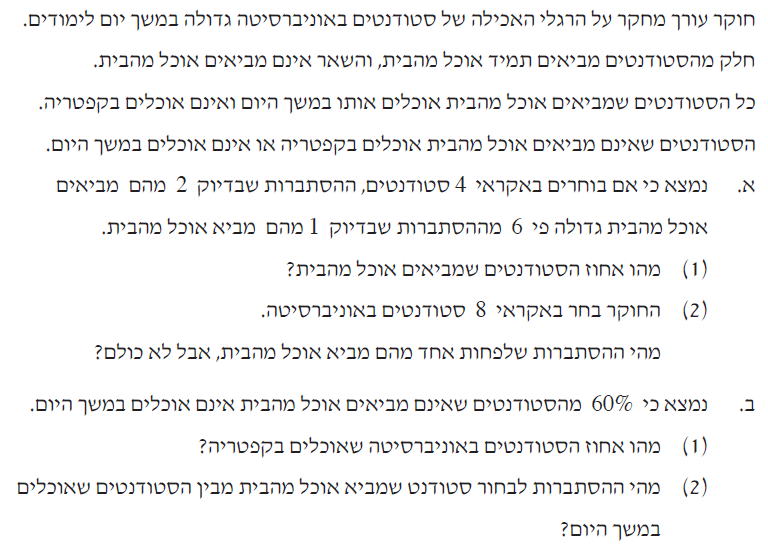
\includegraphics[width=\textwidth]{summer-2015b-3}
\end{center}

סעיף א
$(1)$.
השאלה שואלת רק על המביאים אוכל מהבית. נסמן
$=b$
ההסתברות להביא אוכל מהבית.
\[
{4 \choose 2} b^2(1-b)^2 = 6\cdot {4 \choose 1} b (1-b)^3\,.
\]
פתרון המשוואה הוא 
$b=\frac{4}{5}$.

סעיף א
$(2)$.
"לפחות אחד אבל לא כולם" היא המשלים ל-"לא אפס ולא כולם":
\[
1-\left(\frac{1}{5}\right)^8+\left(\frac{4}{5}\right)^8=0.8322\,.
\]

סעיף ב
$(1)$.
איור~
\L{\ref{fig.summer-2015b.1}}
מראה את עץ ההסתברויות. התשובה מתקבלת מהמסלול המכיל את "אוכל בקפטריה":
\[
\frac{1}{5}\cdot \frac{6}{10} = \frac{2}{25}\,.
\]

\begin{figure}[bt]
\begin{center}
\selectlanguage{english}
\begin{tikzpicture}
[grow=right,
level 1/.append style={level distance=3cm,sibling distance=6em},
level 2/.append style={text width=1cm,level distance=4cm,sibling distance=4em}]
\node[text width=1cm] {} % root
child {
  node {$\frac{4}{5}$}
    edge from parent node[below,xshift=-5mm,yshift=-2mm] {\R{מביא מהבית}}
}
child { 
  node {$\frac{1}{5}$}
    child {
      node {$\frac{6}{10}$}
      edge from parent node[below,xshift=5mm,yshift=-1mm] {\R{אוכל בקפטריה}}
    }
    child {
      node {$\frac{4}{10}$}
      edge from parent node[above,xshift=5mm,yshift=1mm] {\R{לא אוכל}}
    }
    edge from parent node[above,xshift=-4mm,yshift=3mm] {\R{לא מביא מהבית}}
};
\end{tikzpicture}
\selectlanguage{hebrew}
\caption{עץ ההסתברויות של אפשרויות האכילה}\label{fig.summer-2015b.1}
\end{center}
\end{figure}

סעיף ב
$(2)$.
המילה
\textbf{מבין}
מכוונת להסתברות מותנית, כאשר קבוצת "מביא אוכל" היא תת-קבוצה של "אוכלים" והחישוב מצטמטם:
\[
\begin{array}{c}
P(\textrm{\R{מביא אוכל}} / \textrm{\R{אוכלים}})=\\\\
\displaystyle\frac{
P(\textrm{\R{מביא אוכל}} \cap \textrm{\R{אוכלים}})
}
{P(\textrm{\R{אוכלים}})}=\\\\
\displaystyle\frac{
P(\textrm{\R{מביא אוכל}})
}
{P(\textrm{\R{אוכלים}})}\,.
\end{array}
\]
נשתמש בתשובה של סעיף הקודם ונקבל את התשובה:
\[
\frac{4/5}{22/25}=\frac{10}{11}\,.
\]

%%%%%%%%%%%%%%%%%%%%%%%%%%%%%%%%%%%%%%%%%%%%%%%%%%%%%%%%%%%%%%%%%%%
\newpage

\textbf{\R{
חורף תשע"ד
}}
\begin{center}
\selectlanguage{english}
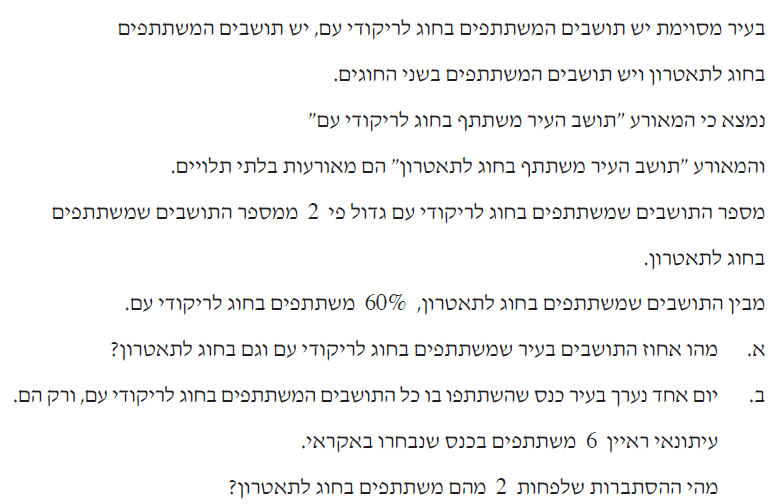
\includegraphics[width=.9\textwidth]{winter-2014-3}
\end{center}

נסמן
$=T$
מספר המשתתפים בתאטרון,
$=R$
מספר המשתתפים בריקודי עם. המילה 
\textbf{מבין}
מכוון להתסברות מותנית. נתון
$P(R/T)=0.6$,
אבל נתון שהסתברויות של שני האירועים בלתי תלויים ולכן:
\[
0.6=P(R/T)=\frac{P(R\cap T)}{P(T)}=\frac{P(R)\cdot P(T))}{P(T)}=P(R)\,.
\]
ביחד עם הנתון
$P(R)=2P(T)$
נתחיל למלא את הטבלה:
\begin{center}
\selectlanguage{english}
\begin{tikzpicture}[scale=1.25]
\draw (0,0) grid (3,3);
\node at (2.5,3.3) {$\bm{T}$};
\node at (1.5,3.3) {$\bover{T}$};
\node at (3.3,2.5) {$\bm{R}$};
\node at (3.3,1.5) {$\bover{R}$};
\node at (0.5,2.5) {$0.60$};
\node at (2.5,0.5) {$0.30$};
\end{tikzpicture}
\end{center}
שבו נסתמך על העובדה של האירועים בלתי תלויים ונקבל:
\[
P(R\cap T)=P(R)\cdot P(T)=0.6\cdot 0.3=0.18\,,
\]
ואז יש לנו מספיק נתונים למלא את הטבלה:
\begin{center}
\selectlanguage{english}
\begin{tikzpicture}[scale=1.25]
\draw (0,0) grid (3,3);
\node at (2.5,3.3) {$\bm{T}$};
\node at (1.5,3.3) {$\bover{T}$};
\node at (3.3,2.5) {$\bm{R}$};
\node at (3.3,1.5) {$\bover{R}$};
\node at (2.5,2.5) {$0.18$};
\node at (0.5,2.5) {$0.60$};
\node at (1.5,2.5) {$0.42$};
\node at (0.5,1.5) {$0.40$};
\node at (0.5,0.5) {$1.0$};
\node at (1.5,0.5) {$0.70$};
\node at (2.5,0.5) {$0.30$};
\node at (1.5,1.5) {$0.28$};
\node at (2.5,1.5) {$0.12$};
\end{tikzpicture}
\end{center}
סעיף א. כבר חישבנו ש-%
$P(R\cap T)=0.18$.

סעיף ב. "כל התושבים המשתתפים בחוג לריקודי עם, ורק הם". ניסוח אחר שמכוון להסתברות מותנית. אם ידוע שתושב משתתף בריקודי עם, ההסתברות שהוא משתתף גם בתאטרון היא
$P(T/R) = P(T) = 0.3$,
כאשר שוב השתמשנו בנתון שהאירועים בלתי תלויים. כדי לחשב "לפחות שניים" עדיף לחשב את המשלים לאפס או אחד":
\[
1-{6\choose 0}(0.3)^0(0.7)^6 +{6\choose 1}(0.3)^1(0.7)^5=0.5798\,.
\]

%%%%%%%%%%%%%%%%%%%%%%%%%%%%%%%%%%%%%%%%%%%%%%%%%%%%%%%%%%%%%%%%%%%


\textbf{\R{
קיץ תשע"ד, מועד א
}}

\begin{center}
\selectlanguage{english}
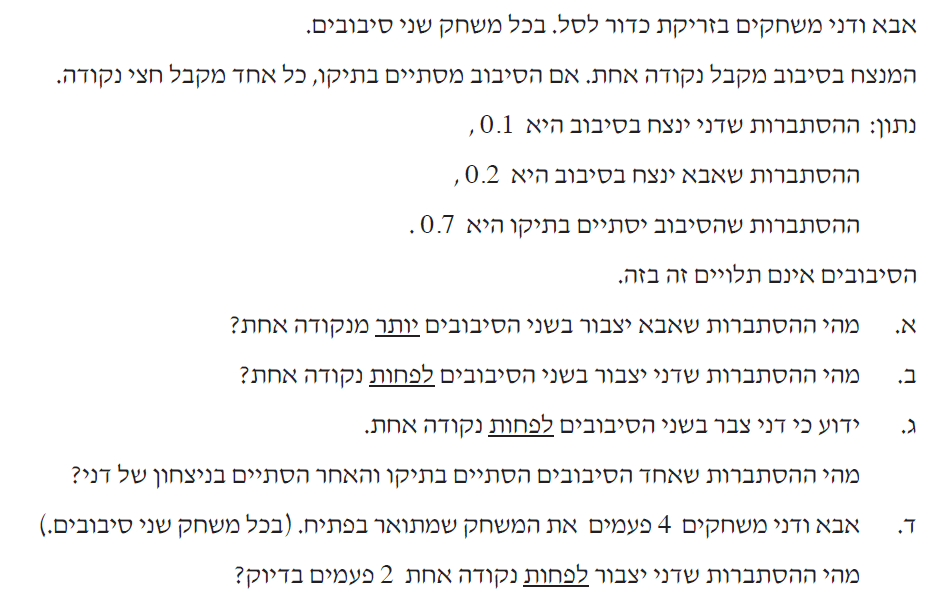
\includegraphics[width=.9\textwidth]{summer-2014a-3}
\end{center}

סעיף א. איור~
\L{\ref{fig.summer-2015a.1}}
מראה את צבירת הנקודות של אבא בשני הסיבובים. באיור, מעברים מסודרים עם אבא למעלה, דני באמצע ותיקו למטה. המצבים בהם אבא צובר
\textbf{יותר}
מנקודה אחת מסומנים בכוכבית. ההסתברות של האירוע היא:
\[
0.2\cdot 0.2 \,+\, 0.2\cdot 0.7 \,+\, 0.7\cdot 0.2 \,=\,0.32\,.
\]

\begin{figure}
\begin{center}
\selectlanguage{english}
\begin{tikzpicture}
[grow=right,
level 1/.append style={font=\sffamily,level distance=3cm,sibling distance=8em},
level 2/.append style={font=\sffamily,level distance=4cm,sibling distance=3em}]
\node[left] {$0$} % root
child {
  node[right] {$\frac{1}{2}$}
    child {
      node[right] {$1$}
      edge from parent node[below,yshift=-1mm] {$0.7$}
    }
    child {
      node[right] {$\frac{1}{2}$}
      edge from parent node[below,xshift=4mm] {$0.1$}
    }
    child {
      node[right] {$1\frac{1}{2}\quad *$}
      edge from parent node[above,yshift=1mm] {$0.2$}
    }
    edge from parent node[below,yshift=-3mm] {$0.7$}
}
child {
  node[right] {$0$}
    child {
      node[right] {$\frac{1}{2}$}
      edge from parent node[below,yshift=-1mm] {$0.7$}
    }
    child {
      node[right] {$0$}
      edge from parent node[below,xshift=4mm] {$0.1$}
    }
    child {
      node[right] {$1$}
      edge from parent node[above,yshift=1mm] {$0.2$}
    }
    edge from parent node[below] {$0.1$}
}
child {
  node[right] {$1$}
    child {
      node[right] {$1\frac{1}{2}\quad *$}
      edge from parent node[below,yshift=-1mm] {$0.7$}
    }
    child {
      node[right] {$1$}
      edge from parent node[below,xshift=4mm] {$0.1$}
    }
    child {
      node[right] {$2\quad *$}
      edge from parent node[above,yshift=1mm] {$0.2$}
    }
    edge from parent node[above,yshift=3mm] {$0.2$}
};
\end{tikzpicture}
\selectlanguage{hebrew}
\caption{עץ ההסתברויות של המשחקים: צבירת נקודות של אבא}\label{fig.summer-2015a.1}
\end{center}
\end{figure}

סעיף ב. איור~
\L{\ref{fig.summer-2015b.1}}
מראה את צבירת הנקודות של דני בשני הסיבובים. המצבים בהם דני צובר 
\textbf{לפחות}
נקודה אחת מסומנים בכוכבית. ההסתברות של האירוע היא:
\[
0.2\cdot 0.1 \,+\,0.1\cdot 0.2 \,+\, 0.1\cdot 0.1 \,+\,0.1\cdot 0.7 \,+\, 0.7\cdot 0.1\,+\,0.7\cdot 0.7\,=\,0.68\,.
\]

\begin{figure}
\begin{center}
\selectlanguage{english}
\begin{tikzpicture}
[grow=right,
level 1/.append style={font=\sffamily,level distance=3cm,sibling distance=8em},
level 2/.append style={font=\sffamily,level distance=4cm,sibling distance=3em}]
\node[left] {$0$} % root
child {
  node[right] {$\frac{1}{2}$}
    child {
      node[right] {$1\quad *$}
      edge from parent node[below,yshift=-1mm] {$0.7$}
    }
    child {
      node[right] {$1\frac{1}{2}\quad *$}
      edge from parent node[below,xshift=4mm] {$0.1$}
    }
    child {
      node[right] {$\frac{1}{2}$}
      edge from parent node[above,yshift=1mm] {$0.2$}
    }
    edge from parent node[below,yshift=-3mm] {$0.7$}
}
child {
  node[right] {$1$}
    child {
      node[right] {$1\frac{1}{2}\quad *$}
      edge from parent node[below,yshift=-1mm] {$0.7$}
    }
    child {
      node[right] {$2\quad *$}
      edge from parent node[below,xshift=4mm] {$0.1$}
    }
    child {
      node[right] {$1\quad *$}
      edge from parent node[above,yshift=1mm] {$0.2$}
    }
    edge from parent node[below] {$0.1$}
}
child {
  node[right] {$0$}
    child {
      node[right] {$\frac{1}{2}$}
      edge from parent node[below,yshift=-1mm] {$0.7$}
    }
    child {
      node[right] {$1\quad *$}
      edge from parent node[below,xshift=4mm] {$0.1$}
    }
    child {
      node[right] {$0$}
      edge from parent node[above,yshift=1mm] {$0.2$}
    }
    edge from parent node[above,yshift=3mm] {$0.2$}
};
\end{tikzpicture}
\selectlanguage{hebrew}
\caption{עץ ההסתברויות של המשחקים: צבירת נקודות של דני}\label{fig.summer-2015b.1}
\end{center}
\end{figure}

סעיף ג. המילים
\textbf{ידוע כי}
מכוונות להסתברות מותנית:
\[
\begin{array}{c}
P(\textrm{\R{תיקו אחד, ניצחון אחד}} / \textrm{\R{דני צבר לפחות נקודה אחת}})=\\\\
\displaystyle\frac{
P(\textrm{\R{תיקו אחד, ניצחון אחד}} \cap \textrm{\R{דני צבר לפחות נקודה אחת}})
}
{P(\textrm{\R{דני צבר לפחות נקודה אחת}})}=\\\\
\displaystyle\frac{
P(\textrm{\R{תיקו אחד, ניצחון אחד}})
}
{P(\textrm{\R{דני צבר לפחות נקודה אחת}})}\,.
\end{array}
\]
החיתוך מצטמצם כי באירוע "תיקו אחד, ניצחון אחד", "דני צבר לפחות נקודה אחת". את המכנה חישבנו בסעיף הקודם, וניתן לחשב את המנה על ידי חיבור ההסתברויות של שני מסלולים בעץ:
\[
\frac{0.1\cdot 0.7 \,+\, 0.7\cdot 0.1}{0.68} = .2059\,.
\]

סעיף ד. בסעיף 2 חישבנו את ההסתברות של האירוע בכל סיבוב, ומכאן נשאר רק לחשב לפי נוסחת ברנולי:
\[
{4\choose 2}(0.68)^2 (0.32)^2= 0.2841\,.
\]

%%%%%%%%%%%%%%%%%%%%%%%%%%%%%%%%%%%%%%%%%%%%%%%%%%%%%%%%%%%%%%%%%%%

\newpage

\textbf{\R{
קיץ תשע"ד, מועד ב
}}

\begin{center}
\selectlanguage{english}
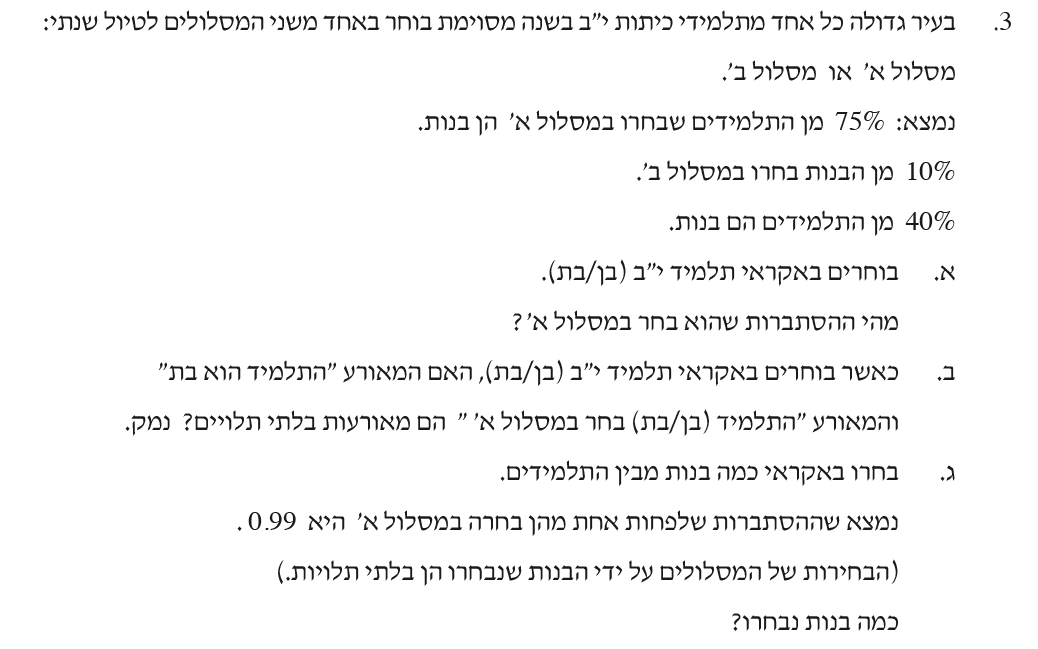
\includegraphics[width=.95\textwidth]{summer-2014b-3}
\end{center}

נמלא את הטבלה ממידע הנתון. נתון ש-% 
$.4$
מהתלמידים הן בנות, ונרשום בתא למטה מימין. 
$10\%$
מהם בחרו במסלול ב, ולכן נרשום את
$.1\times .4=.04$
בתא מעל לתא עם הנתון הראשון. נמשיך ונמלא את התא מעליו בהסתברות המשלימה
$.4-.04=.36$.
הנתון האחרון הוא ש-%
$75\%$
מהתלמידים שבחרו במסלול א הן בנות:
$.75 \cdot \aleph = .36$,
ולכן 
$.48$
מהתלמידים בחרו מסלול א. ניתן למלא את שאר התאים בטלבה לפי משלימים.
\begin{center}
\selectlanguage{english}
\begin{tikzpicture}[scale=2.2]
\draw (0,0) grid (3,3);
\node at (2.5,3.3) {\sffamily\bfseries \R{בנות}};
\node at (1.5,3.3) {\sffamily\bfseries \R{בנים}};
\node at (3.3,2.5) {\sffamily\bfseries \R{א}};
\node at (3.3,1.5) {\sffamily\bfseries \R{ב}};
\node at (2.5,2.7) {$.4-.04=$};
\node at (2.5,2.3) {$.36$};
\node at (0.5,2.7) {$.36/.75=$};
\node at (0.5,2.3) {$.48$};
\node at (1.5,2.7) {$.48-.36=$};
\node at (1.5,2.3) {$.12$};
\node at (0.5,1.7) {$1-.48=$};
\node at (0.5,1.3) {$.52$};
\node at (0.5,0.5) {$1$};
\node at (1.5,0.7) {$1-.4=$};
\node at (1.5,0.3) {$.6$};
\node at (2.5,0.7) {\sffamily\bfseries \R{נתון}};
\node at (2.5,0.3) {$0.4$};
\node at (1.5,1.7) {$.52-.04=$};
\node at (1.5,1.3) {$.48$};
\node at (2.5,1.7) {$.1\times .4=$};
\node at (2.5,1.3) {$.04$};
\end{tikzpicture}
\end{center}
בצורה יותר מפורשת תוך שימוש בהסתברות מותנית:
\[
0.1 = P(\textrm{\R{מסלול ב}} / \textrm{\R{בנות}})=
\displaystyle\frac{
P(\textrm{\R{מסלול ב}} \cap \textrm{\R{בנות}})
}
{P(\textrm{\R{בנות}})}=
\displaystyle\frac{
P(\textrm{\R{מסלול ב}} \cap \textrm{\R{בנות}})
}
{0.4}\,.
\]
מכאן ש:
\[
P(\textrm{\R{מסלול ב}} \cap \textrm{\R{בנות}})
=0.4\cdot 0.1= 0.04\,,
\]
וערך זה מופיע בטבלה בתא המתאים. לפי הסתברות משלימה:
\[
P(\textrm{\R{מסלול א}} \cap \textrm{\R{בנות}}) 
= 0.40-0.04=0.36\,.
\]
נמשיך עם הנתון הנוסף:
\[
0.75 = P(\textrm{\R{בנות}} / \textrm{\R{מסלול א}})=
\displaystyle\frac{
P(\textrm{\R{בנות}} \cap \textrm{\R{מסלול א}})
}{P(\textrm{\R{מסלול א}})}=\frac{0.36}{P(\textrm{\R{מסלול א}})}\,.
\]
מכאן ש:
\[
P(\textrm{\R{מסלול א}})=\frac{0.36}{0.75}=0.48\,.
\]
וערך זה מופיע בטבלה בתא המתאים.

סעיף א. הסעיף מבקש
$P(\textrm{\R{מסלול א}})$
וחישבנו שערכו 
$0.48$.
לכאורה, נראה שמדובר בהסתברות מותנית, אבל מה שידוע הוא שבחרנו תלמיד כלשהו, וברור שההסתברות היא אחת כי כל בחירה היא בחירה של תלמיד. הדבר מודגש בהערה בסוגריים )בן/בת(.

סעיף ב.
\begin{eqnarray*}
P(\textrm{\R{התלמיד הוא בת}} \cap \textrm{\R{מסלול א}}) &=& 
0.36\\
P(\textrm{\R{התלמיד הוא בת}}) \cdot P(\textrm{\R{מסלול א}})
&=&0.4 \cdot 0.48 = 0.192\,,
\end{eqnarray*}
ולכן האירועים
\textbf{אינם}
בלתי תלויים.

סעיף ג. כדי לחשב
\textbf{לפחות אחת},
נחשב שת ההסתברות המשלימה לאף אחת. ההסתברות שבת לא תבחר מסלול א היא ההסתברות שהיא בתחר מסלול ב.
\[
P(\textrm{\R{מסלול ב}} / \textrm{\R{בת}})=
\displaystyle\frac{
P(\textrm{\R{מסלול ב}} \cap \textrm{\R{בת}})
}{P(\textrm{\R{בת}})}
=\frac{0.04}{0.4}=0.1\,,
\]
כאשר ההסתברויות בנוסחה נלקחו מהטבלה. כעת עלינה לפתור את המשוואה:
\[
(0.1)^n=1-0.99=0.01\,.
\]
וברור ש-%
$n=2$.
%%%%%%%%%%%%%%%%%%%%%%%%%%%%%%%%%%%%%%%%%%%%%%%%%%%%%%%%%%%%%%%%%%%

\newpage

\begin{center}
\textbf{סיכום}
\end{center}

\begin{itemize}
\item
\textbf{קרא בזהירות את השאלה}. 
לעתים השאלות ארוכות )בחינה של
\textbf{קיץ תשע"ה א}, \textbf{קיץ תשע"ח ב}(
וחשוב להבין את המשמעות של כל פסקה.

%%%%%%%%%%%%%%%%%%%%%%%%%%%%%%%%%%%%

\item
כמעט כל הבחינות מכילות שאלות על 
\textbf{להסתברות מותנת}.
ניסוחים רבים מכוונים להסתברות מותנית וחשוב להכיר אותם!

\begin{itemize}
\item
הניסוח השכיח ביותר משתמש במילים
\textbf{אם ידוע ש-},
למשל, בבחינה של
\textbf{קיץ תשע"ו ב}:
"חשב את ההסתברות 
$\ldots$,
\textbf{אם ידוע ש-}",
או בבחינה של
\textbf{קיץ תשע"ז א}: "%
\textbf{ידוע ש-}
$\ldots$. 
\textbf{מהי ההסתברות}
$\ldots$. "

\item
בבחינה של
\textbf{חורף תשע"ז}
כתוב "%
\textbf{אם} $\ldots$ ,
\textbf{מהי ההסתברות} $\ldots$".
לא לגמרי ברור שלמילה "אם" יש משמעות של "אם ידוע", אבל זאת הכוונה.
\item
הניסוח בבחינה של
\item
בבחינה של
\textbf{קיץ תשע"ה ב}
כתוב "%
\textbf{מה ההסתברות לבחור} $\ldots$
\textbf{מבין} $\ldots$".

\item
בבחינה של 
\textbf{קיץ תשע"ח א}
הניסוח הוא: "%
$\ldots X\%$
נעזרו 
$\ldots$.
$\displaystyle\frac{k}{n}$
\textbf{מהם}
עברו את הבחינה".

\item
בבחינה של 
\textbf{חורף תשע"ד}
יש ניסוח אחר:
\textbf{כל התושבים המשתתפים ב-} $\ldots$,
\textbf{ורק הם}.
\end{itemize}

%%%%%%%%%%%%%%%%%%%%%%%%%%%%%%%%%%%%

\item
כאשר יש חיתוך בחישוב של הסתברות מותנת, לעתים קרובות ניתן לפשט את החישוב. בבחינה של
\textbf{קיץ תשע"ז א}
יש לחשב
$P(D=4\cap D\ge 3)$,
אבל אם ערך גדול או שווה
$3$
\textbf{וגם}
שווה ל-%
$4$,
אז הוא שווה ל-%
$4$, 
ולכן מספיק לחשב
$P(D=4)$.

%%%%%%%%%%%%%%%%%%%%%%%%%%%%%%%%%%%%

\item
כאשר יש חיתוך בין שני אירועים בלתי תלויים, חישוב ההסתברות המותנית מצטמצם )בחינה של
\textbf{קיץ תשע"ה א}(:
\[
\renewcommand{\arraystretch}{2.4}
\begin{array}{l}
\displaystyle\frac{
P(\textrm{\R{סכום זוגי}} \cap \textrm{\R{ספרה ראשונה זוגית}})
}{P(\textrm{\R{ספרה ראשונה זוגית}})}=\\
\displaystyle\frac{
P(\textrm{\R{סכום זוגי}}) \cdot P(\textrm{\R{ספרה ראשונה זוגית}})
}
{P(\textrm{\R{ספרה ראשונה זוגית}})}=\\
P(\textrm{\R{סכום זוגי}})
\,.
\end{array}
\]
\vspace{-4ex}
%%%%%%%%%%%%%%%%%%%%%%%%%%%%%%%%%%%%

\item
בבחינה של 
\textbf{חורף תשע"ד}
נתון
$P(T/R)$
וגם נתון ששני אירועים הם
\textbf{בלתי תלויים}.
החיתוך שווה למכפלת ההסתברויות, ולכן ההסתברות הידועה מצטצמת ונקבל
$P(T)=P(T/R)$.

%%%%%%%%%%%%%%%%%%%%%%%%%%%%%%%%%%%%

\item
המילה 
\textbf{בדיוק}
מכוונת לחישוב אחד של נוסחת ברנולי, כי נתון כמה "הצלחות" צריכות להיות וגם כמה "כשלונות". מקרה מעניין נמצא בבחינה של
\textbf{קיץ תשע"ח ב}
כאשר נתון שההסתברות לקבל 
$60$
שווה להסתברות לקבל
$100$.
נתון גם שיש שלוש הצלחות מתוך חמש )%
$20$
נקודות כל אחת(, אז ההסתברות לקבל שני "כשלונות" )%
$20$
נקודות כל אחת( צריכה להיות שווה להסתברות לקבל שתי "הצלחות" )%
$20$
נקודות כל אחת(.

%%%%%%%%%%%%%%%%%%%%%%%%%%%%%%%%%%%%

\item
בבחינה של
\textbf{קיץ תשע"ז א}
כתוב "%
\textbf{בוחרים באקראי}
$\ldots$,
\textbf{עד של-}
$3$
מהם
\textbf{בדיוק}
יש קלנועית". מהמילים "עד ש-" אפשר להבין שמפסיקים את הבחירה האקראית כאשר הבחירה 
\textbf{האחרונה} 
היא "הצלחה". במקרה זה נשארו שתי "הצלחות" שיש לחשב את ההסתברות שלהן לפי נוסחת ברנולי, ואז להכפיל בהסתברות של "הצלחה" בבחירה האחרונה:
\[
\overbrace{\pm\;\pm\;\pm\;\pm\;\pm}^{2/5}\quad\quad \overbrace{+}^{1/1}\,.
\]
דרך אחרת לחשב שאלות מסוג זה הודגמה בבחינה של
\textbf{חורף תשע"ח},
שם השתמשנו בעובדה שהטלות הקוביה הן בלתי תלויות ולכן ההסתברות של ההטלה הראשונה מצטמצמת בחישוב ההסתברות המותנית.

%%%%%%%%%%%%%%%%%%%%%%%%%%%%%%%%%%%%

\item
בבחינה של
\textbf{קיץ תשע"ז ב}
הביטוי "%
\textbf{מוציאים באקראי},
$\ldots$",
ובהמשך הביטוי "%
\textbf{שוב מוציאים באקראי}
$\ldots$"
מכוון לשימוש בעץ כדי לתאר את הבחירה הסדרתית.

%%%%%%%%%%%%%%%%%%%%%%%%%%%%%%%%%%%%

\item
בבחינה של
\textbf{קיץ תשע"ח א},
הניסוח "%
\textbf{לפחות אחת}
משתי הטענות 
$I, II$"
שהאירוע קורה אם קורה אחד מהאירועים
$I, II$,
\textbf{או שניהם},
המסומן 
$I \cup II$.
יש שתי דרכים לחשב את ההסתברות: על ידי חיבור ההסתברות של שני האירועים וחיסור האירוע המשותף כדי לקזז את הספירה הכפולה, או לחבר את האירוע המשותף עם האירועים של אחד ולא השני.
\begin{eqnarray*}
P(I \cup II) &=& P(I) + P(II) - P(I \cap II)\\
P(I \cup II) &=& P(I/ II) + P(II/ I) + P(I \cap II)\,.
\end{eqnarray*}
הערכים לחישוב
$P(I \cup II)$
בשתי הדרכים מסומנים בטבלה להלן, כאשר התא המקווקו מופיע פעמיים, פעם כחלק מהאירוע
$I$
ופעם כחלק מהאירוע
$II$:
\begin{center}
\selectlanguage{english}
\begin{tikzpicture}[scale=1.4]
\begin{scope}
\draw (0,0) grid (3,3);
\node at (2.5,3.3) {$\bm{I}$};
\node at (1.5,3.3) {$\bover{I}$};
\node at (3.3,2.5) {$\bm{II}$};
\node at (3.3,1.5) {$\bover{II}$};
\node at (2.5,2.5) {$I\cap II$};
\node at (2.5,1.5) {$I/ II$};
\node at (1.5,2.5) {$II/ I$};
\draw[ultra thick] (2,2) rectangle +(1,1);
\draw[ultra thick] (1,2) rectangle +(1,1);
\draw[ultra thick] (2,1) rectangle +(1,1);
\end{scope}
\begin{scope}[xshift=5cm]
\draw (0,0) grid (3,3);
\node at (2.5,3.3) {$\bm{I}$};
\node at (1.5,3.3) {$\bover{I}$};
\node at (3.3,2.5) {$\bm{II}$};
\node at (3.3,1.5) {$\bover{II}$};
\node at (2.5,2.5) {$I\cap II$};
\node at (2.5,0.5) {$I$};
\node at (0.5,2.5) {$II$};
\draw[ultra thick] (0,2) rectangle +(1,1);
\draw[ultra thick] (2,0) rectangle +(1,1);
\draw[ultra thick,dashed] (2,2) rectangle +(1,1);
\end{scope}
\end{tikzpicture}
\end{center}

%%%%%%%%%%%%%%%%%%%%%%%%%%%%%%%%%%%%

\item
בבחינה של
\textbf{חורף תשע"ו}
נתון ההסתברות
$p$
ש-"לא יזכה
\textbf{באף משחק}
$M$
מתוך 
$n$
משחקים". גם בבחינה של 
\textbf{קיץ תשע"ח ב}
צריכים לחשב את ההסבתרות של תשובה נכונה 
\textbf{לכל}
שאלה או תשובה נכונה
\textbf{לאף אחת}
מהשאלות.  אין צורך להשתמש בנוסחת ברנולי במלואו:
\[
{n \choose k}p^k(1-p)^{n-k}\,.
\]
אם
$k=0$
או
$k=n$,
הבחירה של
$k$
מתוך 
$n$
שווה אחד, וההסתברות המשלימה מועלה לחזקת אפס והגורם הוא גם כן שווה לאחד. נשאר רק גורם אחד 
$p^k$.

%%%%%%%%%%%%%%%%%%%%%%%%%%%%%%%%%%%%

\item
בבחינות של 
\textbf{קיץ תשע"ו א, ב}
יש שלוש תוצאות אפשרויות במקום שתיים. סכום ההסתברויות חייב להיות אחד, ולכן כאשר מחשבים משלים להסתברות אחת, יש להחסיר את שתי ההסתברויות האחרות. בבחינה של מועד ב: ההסתברות לתיקו היא אחד פחות ההסתברות שיעל תנצח פחות ההסתברות אנה תנצח:
\[
P(\textrm{\R{תיקו}}) =
1 - (P(\textrm{\R{יעל}})+
P(\textrm{\R{אנה}})) = 
1 - P(\textrm{\R{יעל}})-
P(\textrm{\R{אנה}}) \,.
\]
\end{itemize}

\end{document}
